\chapter{Implementacija}
\label{ch:implementacija}


Ovo poglavlje opisuje kako su \v{c}etiri efekta zasnovana na pra\'cenju zraka i zajedni\v{c}ki denoiser implementirani u Snowstorm engine-u, sa te\v{z}i\v{s}tem na samom pra\'cenju zraka i njegovoj ceni, a ne na svakom podsistemu engine-a.

\section{Snowstorm Engine (pregled)}
\label{sec:engine}

Snowstorm je Vulkan engine koji je autor napisao od nule. Ovaj rad ga koristi kao doma\'cina za prolaze sa pra\'cenjem zraka i ne smatra sam engine doprinosom. Sistem entiteta i komponenti (ECS) zasnovan na EnTT-u proizvodi renderski posao za svaki frejm. Sloj \texttt{Render/} nezavisan od bekenda le\v{z}i nad Vulkan RHI slojem (volk, Vulkan Memory Allocator, spirv-reflect za rasporede deskriptora) u \texttt{Platform/Vulkan/}, \v{s}ejderi su HLSL kompajliran u SPIR-V preko dxc-a, a ImGui editor sadr\v{z}i CVar konzolu i prikaz performansi (Odeljak~\ref{sec:alati}).

Jedini deo od klju\v{c}nog zna\v{c}aja za RT putanju je bindless model deskriptora, koji omogu\'cava da jedna rutina za \v{s}ejdiranje pogotka indeksira temena, indekse i materijal bilo kog mesha celobrojnim indeksom, umesto kroz resurse vezane za taj konkretan poziv crtanja (Odeljak~\ref{sec:efekti}): svaki mesh izla\v{z}e svoje bafere temena i indeksa preko adrese ure\dj{}aja, a tabela geometrije po instanci, indeksirana preko \texttt{instanceCustomIndex}, omogu\'cava \v{s}ejderu pogotka da u trenutku pra\'cenja dobavi atribute pogo\dj{}enog trougla i njegov materijal. Vulkan fizi\v{c}ki ure\dj{}aj bira se pri pokretanju po indeksu ili imenu kroz CVar, pa isti binarni fajl radi na obe grafi\v{c}ke kartice, od \v{c}ega zavisi me\dj{}uvendorska evaluacija iz Glave~\ref{ch:analiza}.

\section{Graf renderovanja i struktura frejma}
\label{sec:rendergraph}

Renderer je organizovan kao \texttt{RenderGraph}: prolazi se dodaju redom, svaki deklari\v{s}e teksture koje \v{c}ita i pi\v{s}e, a graf iz tih deklaracija izvodi i Vulkan barijere rasporeda izme\dj{}u njih i DAG zavisnosti (\texttt{BuildDependencies}). Redosled deklaracije je po konstrukciji ispravan topolo\v{s}ki redosled, pa izvedene ivice nikad ne menjaju \v{s}ta je ispravno, ve\'c samo \v{s}ta bi bilo slobodno za preme\v{s}tanje. Svako merenje u ovom radu izvr\v{s}ava se u redosledu deklaracije.

Graf mo\v{z}e i da rasporeduje prema tim ivicama umesto da ih samo sledi: lance sa pra\'cenjem zraka grupi\v{s}e u jedan neprekinut compute niz, da bi se blok mogao premestiti na asinhroni red. Obe polovine su izgra\dj{}ene i obe su izmerene kao neto negativne: samo preure\dj{}ivanje pomera vreme celog frejma za 0.2\%, unutar raspona izme\dj{}u pokretanja, a asinhroni red ko\v{s}ta $+0.675$ ms, $+4.1\%$, jer ra\v{c}vanje, spajanje i prenosi vlasni\v{s}tva nad porodicom redova prema\v{s}uju 1.1\% rasterskog posla koji je na raspolaganju za preklapanje. Grupisanje compute posla je standardan savet za koji ovaj frejm nema \v{c}ime da se isplati, pa obe zastavice ostaju isklju\v{c}ene, a raspored je mogu\'cnost grafa, a ne svojstvo bilo kog broja iz Glave~\ref{ch:analiza}. DAG iza njega nosi jedno upozorenje koje vredi navesti jer bi ograni\v{c}ilo svaku budu\'cu upotrebu: prate se samo teksture, pa prolaz koji dira strukturu ubrzanja, bindless tabelu ili bafer ima stvaran zahtev za redosledom koji nijedna ivica ne bele\v{z}i. CVar \texttt{render.graph.dumpdeps} prijavljuje koji prolazi izgledaju neograni\v{c}eno, \v{c}ime ta praznina ostaje vidljiva umesto latentna.

Svaki prolaz je obavijen imenovanim GPU timestamp opsegom (\texttt{BeginGpuScope}), a ta imena su redovi Tabele~\ref{tab:pass-cost} u Glavi~\ref{ch:analiza}, pa su struktura grafa i najfinija raspolo\v{z}iva granularnost merenja jedno te isto. Cene po efektu u Tabeli~\ref{tab:cena} namerno su grublje, razlike celog frejma umesto o\v{c}itavanja opsega, jer podrazumevana putanja senki nema sopstveni opseg.

Slika~\ref{fig:overview} prikazuje frejm u obrisu, a Tabela~\ref{tab:framegraph} daje deklarisani redosled po viewport-u.

\begin{figure}[tbp]
\centering
\begin{tikzpicture}[>={Stealth[]}, font=\small, node distance=0mm,
  stage/.style={draw, rounded corners, align=center, minimum height=8mm, inner xsep=3pt},
  rt/.style={stage, fill=black!7, minimum width=2.3cm},
  lbl/.style={font=\scriptsize\itshape}]

  \node[stage] (gbuf) at (0,0) {G-bafer\\[-1pt]\footnotesize dubina + normale};

  \node[rt, right=9mm of gbuf, yshift=13mm] (gi) {GI\\[-1pt]\footnotesize pola rez.};
  \node[rt, right=9mm of gbuf] (ao) {AO\\[-1pt]\footnotesize pola rez.};
  \node[rt, right=9mm of gbuf, yshift=-13mm] (refl) {Refleksije\\[-1pt]\footnotesize puna rez.};

  \node[stage, right=9mm of ao, minimum height=30mm, text width=2.1cm] (fwd)
    {Forward\\\v{s}ejdiranje\\[2pt]\footnotesize + inline\\\footnotesize zraci senki};
  \node[stage, right=8mm of fwd, text width=1.7cm] (post) {TAA\\tonemap\\post};

  \foreach \t in {gi,ao,refl} {
    \draw[->] (gbuf.east) -- (\t.west);
    \draw[->] (\t.east) -- (fwd.west);
  }
  \draw[->] (fwd.east) -- (post.west);

  \node[lbl, above=1mm of gi] {pra\'cenje $\rightarrow$ akumulacija $\rightarrow$ filtriranje $\rightarrow$ upsample};
  \node[lbl, below=1mm of refl] {osen\v{c}eno sivo = prati zrake};
\end{tikzpicture}
\caption[Frejm u glavnim crtama]{Frejm u glavnim crtama. Rasterizovani G-bafer hrani tri efekta sa pra\'cenjem zraka koja se rekonstrui\v{s}u u teksture pre \v{s}ejdiranja, dok se \v{c}etvrti (senke) prati inline unutar forward prolaza. Svaki sivi lanac ponavlja isti oblik pra\'cenje-pa-akumulacija, \v{s}to omogu\'cava da jedan denoiser slu\v{z}i svima, iako samo efekti sa polovinom rezolucije (GI i AO) dodaju prostorni filter i upsample: refleksije rade u punoj rezoluciji sa podrazumevano isklju\v{c}enim filterom (Odeljak~\ref{sec:denoise-eval}). Tabela~\ref{tab:framegraph} daje isto, prolaz po prolaz.}
\label{fig:overview}
\end{figure}

\begin{table}[tbp]
\caption[Prolazi po frejmu, redom]{Prolazi po frejmu u redosledu izvr\v{s}avanja. Tri efekta se rekonstrui\v{s}u pre \v{s}ejdiranja i ulaze u \texttt{Forward} kao teksture, a senke su izuzetak i prate se inline unutar prolaza \texttt{Forward}. Navedeni post lanac je ono \v{s}to se zaista izvr\v{s}ava: \texttt{render.aa} bira jedan metod anti-aliasinga umesto da ih ulan\v{c}ava (nijedan, FXAA, TAA ili DLAA, neuronska temporalna mre\v{z}a pokrenuta u nativnoj rezoluciji kao temporalni resolve), pa su ta \v{c}etiri alternative i svako merenje ovde fiksira TAA, dok \texttt{render.sharpen} i \texttt{render.scale} stoje na podrazumevanim vrednostima 0 i 1.0, \v{s}to ostavlja prolaze izo\v{s}travanja i upscale-a nezakazanim. Frejm izmeren u Tabeli~\ref{tab:pass-cost} sadr\v{z}i \perfPassCount{} prolaza i nijedan od ta tri nije me\dj{}u njima.}
\label{tab:framegraph}
\centering
\small
\begin{tabular}{@{}>{\raggedright\arraybackslash}p{2.9cm}@{\hspace{4mm}}>{\raggedright\arraybackslash}p{9.4cm}@{}}
\toprule
\textbf{Faza} & \textbf{Prolazi, redom} \\
\midrule
G-bafer & \texttt{DepthNormal} (dubina + geometrijska normala), \texttt{Velocity} (vektori kretanja) \\
\addlinespace[2pt]
GI (1/2 rez.) & \texttt{GI} $\rightarrow$ \texttt{GITemporal} $\rightarrow$ \texttt{GIDenoise} $\rightarrow$ \texttt{GIUpsample} \\
\addlinespace[2pt]
AO (1/2 rez.) & \texttt{AO} $\rightarrow$ \texttt{AOTemporal} $\rightarrow$ \texttt{AODenoise} $\rightarrow$ \texttt{AOUpsample} \\
\addlinespace[2pt]
Refleksije (puna) & \texttt{Reflection} $\rightarrow$ \texttt{ReflectionTemporal} (a-trous filter za refleksije je podrazumevano isklju\v{c}en) \\
\addlinespace[2pt]
\v{S}ejdiranje & \texttt{Forward} (\texttt{DefaultLit}): depth prepass, pa lit \v{s}ejder radi jednom po vidljivom pikselu, nebo, inline zraci senki i kombinovanje sa GI/AO/refleksijama \\
\addlinespace[2pt]
Post & \texttt{TemporalResolve} (TAA) $\rightarrow$ \texttt{PostProcess} (tonemap). \texttt{Upscale} (uklju\v{c}uju\'ci DLAA putanju), \texttt{FXAA} i \texttt{Sharpen} postoje, ali se ne izvr\v{s}avaju ni u jednoj ovde izmerenoj konfiguraciji \\
\addlinespace[2pt]
Merenje & \texttt{Compare}, \texttt{Metrics} (PSNR, SSIM) \\
\bottomrule
\end{tabular}
\end{table}


Tri od \v{c}etiri efekta rade kao compute prolazi \emph{pre} forward prolaza, svaki pi\v{s}e denoisovanu teksturu koju forward \v{s}ejder potom uzorkuje. Kao po\v{c}etnu povr\v{s}inu trebaju G-bafer dubine i normala, pa slede \texttt{DepthNormal}, ali prethode \v{s}ejdiranju. Njihovo izvr\v{s}avanje ispred forward-a omogu\'cava jedno lit kombinovanje (direktno osvetljenje plus uzorkovano indirektno, AO i refleksija) umesto preplitanja pra\'cenja i \v{s}ejdiranja. Ova podela, sa screen-space compute efektima koji hrane forward kombinovanje, prati na\v{c}in na koji hibridni renderi poput Unreal-ovog Lumen-a razdvajaju svoje screen prolaze od osvetljenja pogodaka.

Senke su namerni izuzetak: zrak senke se prati \emph{inline} unutar forward \v{s}ejdera, jednom po svetlu po pikselu, u punoj rezoluciji i bez denoisera izme\dj{}u (Odeljak~\ref{sec:senke}). Test vidljivosti je jedan bit koji je jeftino izra\v{c}unati ta\v{c}no, a skupo rekonstruisati pribli\v{z}no, pa za mali broj svetala odgovor na licu mesta pobe\dj{}uje pisanje bafera, njegovo filtriranje i ponovno \v{c}itanje. Cena je linearan rast sa brojem svetala, \v{s}to alternativna stohasti\v{c}ka putanja iz Odeljka~\ref{sec:senke} treba da re\v{s}i.

GI i AO se prate u polovini rezolucije (\texttt{render.gi.scale}, \texttt{render.ao.scale}, oba podrazumevano 0.5) i bilateralno se upsample-uju pre nego \v{s}to ih forward prolaz uzorkuje, dok se refleksije prate u punoj rezoluciji. Pra\'cenje u polovini rezolucije je najve\'ca pojedina\v{c}na poluga cene za ova dva hemisferna efekta jer \v{c}etvrtina zraka ostaje, a Odeljak~\ref{sec:cena} kvantifikuje \v{s}ta se time dobija. Koji efekti to podnose nije proizvoljno: rekonstrukcija tri piksela od \v{c}etiri iz suseda bezbedna je samo kad se signal sporo menja du\v{z} povr\v{s}ine. Ambijentalna okluzija i difuzno globalno osvetljenje su \v{s}iroki hemisferni proseci, pa susedni pikseli na istom zidu zaista dobijaju skoro isti odgovor, a interpolacija unosi manju gre\v{s}ku od \v{s}uma koji ve\'c postoji. Granica senke je step funkcija, a refleksija zavisi od pogleda, pa susedni piksel tu legitimno mo\v{z}e da vidi ne\v{s}to potpuno druga\v{c}ije, a prepolovljena rezolucija uni\v{s}tava detalj zbog kog se efekat uop\v{s}te isplatilo pratiti umesto zamutiti.

\section{Izgradnja struktura ubrzanja (BLAS/TLAS)}
\label{sec:accel}

Ray query-ji prate zrake kroz dvonivovsku strukturu opisanu u Odeljku~\ref{sec:accel-pregled}. Svaki jedinstveni mesh poseduje jedan BLAS, gradi se lenjo pri prvoj upotrebi i ke\v{s}ira na meshu (\texttt{Mesh::GetOrBuildBLAS}) sa zastavicom \texttt{PREFER_FAST_TRACE} nad neprozirnom geometrijom trouglova referenciranom preko adrese ure\dj{}aja (pozicije R32G32B32, 32-bitni indeksi). Neprozirni meshevi su ozna\v{c}eni sa \texttt{OPAQUE}, pa obilazak preska\v{c}e any-hit fazu, dok materijali sa alfa isecanjem (glTF MASK) pribegavaju minimalnom any-hit alfa testu, osim ako nije dostupan opacity micromap. TLAS dr\v{z}i po jednu instancu za svaki (Transform, Mesh) entitet, a svaka nosi svoju $3\times4$ svetsku transformaciju, masku vidljivosti, adresu svog BLAS-a i \texttt{instanceCustomIndex} postavljen na indeks instance, da bi \v{s}ejder pogotka mogao da razre\v{s}i geometriju iz tabele (Odeljak~\ref{sec:efekti}).

U \texttt{Sponza.world} dvonivovska struktura ne donosi ni\v{s}ta, jer je model autorski postavljen kao jedan neponavljani skup mesheva: 25 instanci nad 25 BLAS-ova, jedan na jedan. \texttt{Sponza-Motion.world} dodaje \v{c}etiri rotiraju\'ca rekvizita iz Odeljka~\ref{sec:motion}, \v{c}etiri transformacije jednog mesha, pa njenih 29 instanci deli 26 BLAS-ova.

TLAS se u celini ponovo gradi u svakom frejmu u kom je scena ozna\v{c}ena kao izmenjena (\texttt{TlasBuildSystem}, u fazi \texttt{PreRender}). Ne postoji putanja osve\v{z}avanja (refit): izmenjen frejm uni\v{s}tava i ponovo gradi strukturu (\texttt{MODE_BUILD_KHR}) iza \v{c}ekanja ure\dj{}aja. Provera izmene izuzima kameru, pa scena sa stati\v{c}nom geometrijom i transformacijama ne gradi TLAS ponovo ni dok se kamera kre\'ce, \v{s}to je uobi\v{c}ajen slu\v{c}aj za benchmark scenu. Potpuna ponovna izgradnja u svakom dinami\v{c}nom frejmu je te\v{z}a od osve\v{z}avanja. To je navedeno kao ograni\v{c}enje u Glavi~\ref{ch:zakljucak}, a izabrano je zbog jednostavnosti implementacije, s obzirom na to da su test scene uglavnom stati\v{c}ne.

\paragraph{Opacity micromap-e za ise\v{c}enu geometriju.} Na ure\dj{}aju koji izla\v{z}e \texttt{VK\_EXT\_opacity\_micromap} (\texttt{render.omm}, podrazumevano uklju\v{c}eno kad je podr\v{z}ano), materijal sa isecanjem umesto toga gradi drugi BLAS, koji nije ozna\v{c}en kao neprozirn i nosi opacity micromap: compute prolaz (\texttt{OmmBake.comp}) pe\v{c}e alfu albeda materijala u klasifikaciju po mikrotrouglu na neprozirno/prozirno/nepoznato, na fiksnom nivou podele. Obilazak potom u hardveru razre\v{s}ava neprozirne i prozirne mikrotrouglove, pa any-hit alfa test radi samo na nepoznatim (ivi\v{c}nim) (Slika~\ref{fig:omm}), dok bez ekstenzije svaki mikrotrougao ise\v{c}enog materijala pla\'ca taj test. Pe\v{c}enje se izvr\v{s}ava jednom po meshu i ke\v{s}ira uz obi\v{c}an BLAS. Po\v{s}to uzorkuje rezidentnu teksturu albeda, odla\v{z}e se dok se ta tekstura ne u\v{c}ita do kraja (placeholder asinhronog u\v{c}itavanja je neproziran, a pe\v{c}enje nad njim trajno bi ke\v{s}iralo pun ise\v{c}ak), a u me\dj{}uvremenu se koristi any-hit rezerva. Podr\v{s}ka zavisi i od drajvera i od hardvera: na RDNA4 GPU kori\v{s}\'cenom ovde Vulkan drajver ne izla\v{z}e ekstenziju uprkos hardveru, dok Blackwell NVIDIA GPU to radi, pa dva vendora iz Glave~\ref{ch:analiza} koriste razli\v{c}ite putanje geometrije za maskirane materijale, uz iste semantike upita nad strukturom ubrzanja.

\begin{figure}[tbp]
\centering
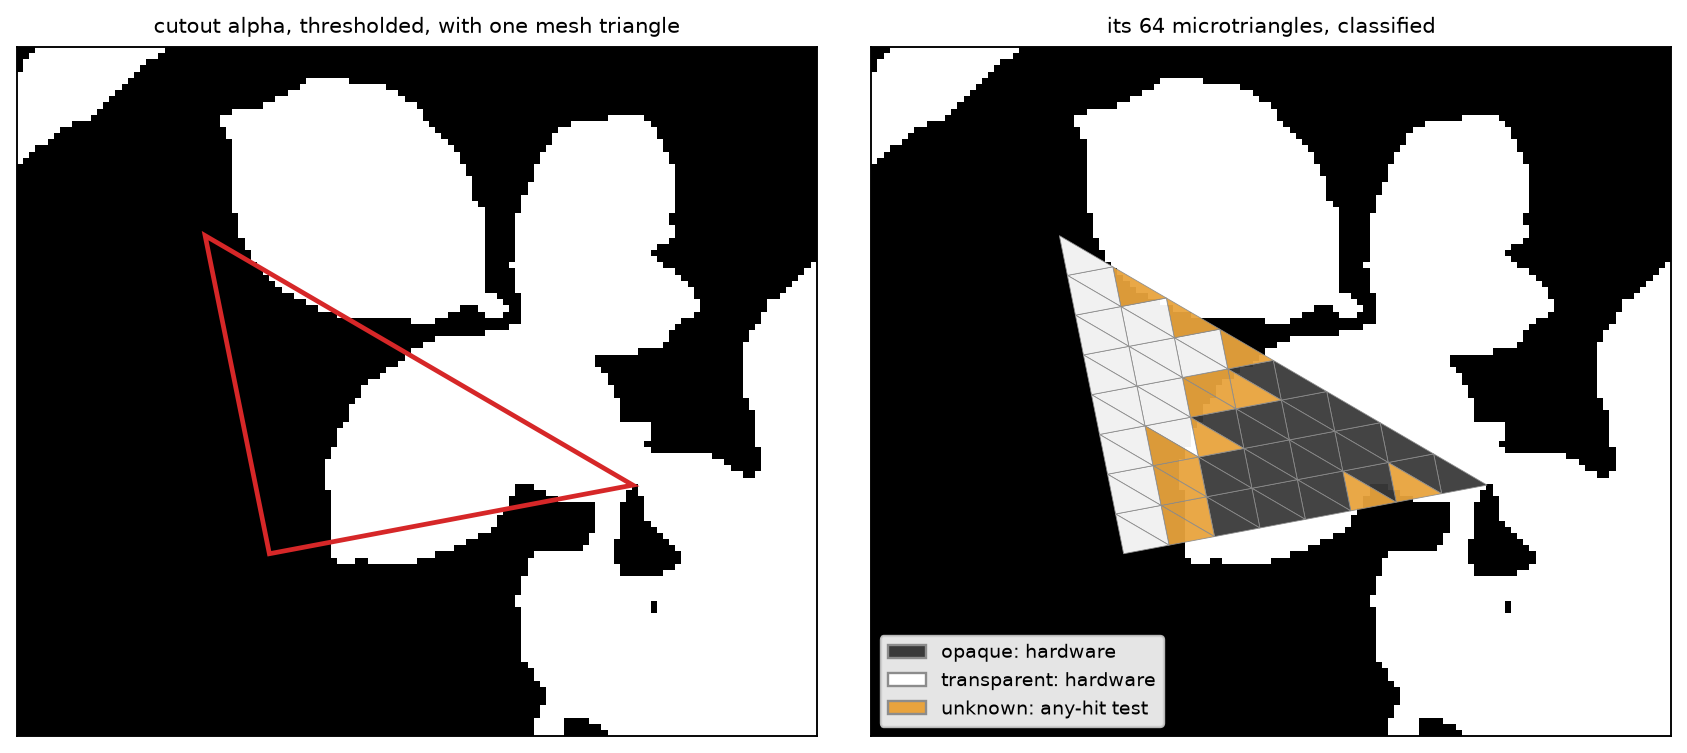
\includegraphics[width=\textwidth]{figures/omm_classify.png}
\caption[Klasifikacija opacity micromap-a ise\v{c}enog trougla]{\v{S}ta pe\v{c}enje proizvodi, za jedan stvarni trougao Sponza materijala sa isecanjem, na isporu\v{c}enom nivou podele. \textbf{Levo:} alfa materijala pragovana na svojoj granici, belo gde zrak poga\dj{}a i crno gde prolazi, sa ocrtanim trouglom. \textbf{Desno:} njegovih \ommTotal{} mikrotrouglova, svaki klasifikovan prema uzorcima u njemu. Samo \ommUnknown{} preseca alfa granicu i ostaje nepoznato, pa je \ommHwPct\% trougla razre\v{s}eno tokom obilaska, a any-hit alfa test radi samo na narand\v{z}astom pojasu. Mikrotrougao se naziva neprozirnim ili prozirnim samo kad se svi uzorci u njemu sla\v{z}u, pa nejasan uvek pada na ta\v{c}an test, te ekstenzija menja cenu obilaska, a ne ono \v{s}to on nalazi.}
\label{fig:omm}
\end{figure}

Engine uklju\v{c}uje \texttt{VK_KHR_ray_query} i \texttt{VK_KHR_acceleration_structure} (plus \texttt{VK_KHR_deferred_host_operations} za izgradnju), ali ne i ekstenziju ray tracing pipeline-a. Ne postoji shader binding table: svako pra\'cenje je \texttt{RayQuery} objekat kreiran unutar ina\v{c}e obi\v{c}nog compute ili fragment \v{s}ejdera.

Tamo gde bi DXR slao hit grupu po geometriji, ovde se ni\v{s}ta ne \v{s}alje: \v{s}ejder dobija tri celobrojne vrednosti i sam mora da prona\dj{}e povr\v{s}inu, vode\'ci indeks instance kroz \texttt{GeoRecord} tabelu na adresi ure\dj{}aja do bafera indeksa i temena mesha i njegovog bindless materijala (Slika~\ref{fig:hitresolve}). Jedna rutina, \texttt{ResolveHit} u \texttt{RTHitShading.hlsli}, stoga razre\v{s}ava \emph{bilo koji} mesh u sceni bez \v{s}ejdera po geometriji i bez ponovnog vezivanja deskriptora, \v{s}to i omogu\'cava da se jedan \texttt{ShadeSurfaceHit} koristi iz sva \v{c}etiri efekta.

\begin{figure}[tbp]
\centering
\begin{tikzpicture}[>={Stealth[]}, font=\small, node distance=4mm,
  box/.style={draw, rounded corners, align=left, inner sep=4pt, text width=4.4cm},
  src/.style={box, fill=black!7}]
  \node[src] (hit) {\textbf{Pogo\dj{}eni trougao}\\\footnotesize \texttt{instanceId}, \texttt{prim},
    \texttt{bary}};
  \node[box, below=8mm of hit] (rec) {\textbf{\texttt{GeoRecord}}\\\footnotesize adrese bafera temena i indeksa, indeks teksture, materijal};
  \node[box, right=16mm of rec] (idx) {\textbf{Bafer indeksa}\\\footnotesize tri indeksa na
    \texttt{IndexAddress + prim*12}};
  \node[box, below=8mm of rec] (vtx) {\textbf{Bafer temena}\\\footnotesize atributi, interpolirani
    barycentrics-ima};
  \node[box, right=16mm of vtx] (tex) {\textbf{Bindless niz tekstura}\\\footnotesize
    \texttt{NonUniformResourceIndex}};
  \node[src, below=8mm of vtx] (out) {\textbf{\texttt{HitSurface}}\\\footnotesize albedo, normala,
    metalnost, hrapavost};
  \draw[->] (hit) -- node[right, font=\scriptsize] {tabela preko adrese} (rec);
  \draw[->] (rec) -- (idx);
  \draw[->] (rec) -- (vtx);
  \draw[->] (idx) -- (vtx);
  \draw[->] (rec.east) to[out=-30, in=30] (tex.north east);
  \draw[->] (tex) -- (out);
  \draw[->] (vtx) -- (out);
\end{tikzpicture}
\caption[Razre\v{s}avanje pogotka kroz bindless tabelu geometrije]{Od pogo\dj{}enog trougla do osen\v{c}ene povr\v{s}ine, bez shader binding table-a. \texttt{RayQuery} vra\'ca samo tri broja, a iz njih \texttt{ResolveHit} sti\v{z}e do geometrije i materijala kroz tabelu indeksiranu preko \texttt{instanceCustomIndex}. Indeks teksture nije uniforman unutar wave-a, pa mora da pro\dj{}e kroz \texttt{NonUniformResourceIndex}.}
\label{fig:hitresolve}
\end{figure}

\section{\v{C}etiri efekta preko inline ray query-ja}
\label{sec:efekti}

Sva \v{c}etiri efekta dele istu osnovnu operaciju: konstruisati zrak, kreirati \texttt{RayQuery} nad TLAS-om scene, izvr\v{s}iti njegovu petlju obilaska i postupiti prema rezultatu. Razlikuju se po \v{c}etiri ose iz Tabele~\ref{tab:effect-params}, od kojih su dve spregnute: efekat kome treba samo odgovor o vidljivosti mo\v{z}e da stane na prvom pogotku, \v{s}to je i jeftiniji obilazak i razlog za\v{s}to mo\v{z}e da priu\v{s}ti manji broj zraka od efekta koji mora da osen\v{c}i ono \v{s}to na\dj{}e.

\begin{table}[tbp]
\caption[Parametri \v{c}etiri efekta]{Kako se \v{c}etiri efekta razlikuju pod istom inline ray query operacijom. Broj zraka i razmera su podrazumevane vrednosti odgovaraju\'cih CVar-ova. ``Prvi pogodak'' je \texttt{RAY\_FLAG\_ACCEPT\_FIRST\_HIT\_AND\_END\_SEARCH}, koji zaustavlja obilazak \v{c}im na\dj{}e bilo kakav presek.}
\label{tab:effect-params}
\centering
\begin{tabular}{lllll}
\toprule
Efekat & zraka/piksel & obilazak & rezultat pogotka & razmera \\
\midrule
senke        & 2 po svetlu & prvi pogodak & vidljivost (0/1)  & 1.0 \\
AO           & 2           & prvi pogodak & okluzija + rastojanje & 0.5 \\
refleksije   & 1           & najbli\v{z}i     & osen\v{c}ena radijansa   & 1.0 \\
GI           & 2           & najbli\v{z}i     & osen\v{c}ena radijansa   & 0.5 \\
\bottomrule
\end{tabular}
\end{table}

Efekti koji \v{s}ejdiraju svoje pogotke (refleksije i GI) dele jednu rutinu, \texttt{ShadeSurfaceHit} u \texttt{RTHitShading.hlsli}, koja razre\v{s}ava pogo\dj{}eni trougao kroz bindless tabelu geometrije i ra\v{c}una jedan odskok, dok senkama i AO treba samo odgovor o vidljivosti i koriste jeftiniji any-hit obilazak. Primarno \v{s}ejdiranje u forward prolazu je standardni metallic-roughness Cook-Torrance model (GGX distribucija, Smith geometrija sa Schlick-GGX aproksimacijom, Schlick Fresnel, Lambertov difuzni \v{c}lan), sa ambijentalnim \v{c}lanom iz prefiltriranog cube mape okru\v{z}enja i unapred izra\v{c}unate tabele BRDF-a.

Sekundarni pogoci se \v{s}ejdiraju jeftinije, namerno: \texttt{ShadeSurfaceHit} ra\v{c}una Lambertov difuzni \v{c}lan skaliran sa $(1 - \text{metallic})$, plus emisivni \v{c}lan povr\v{s}ine i image-based ambijentalno punjenje, bez ikakvog spekularnog re\v{z}nja, pa provodnik vi\dj{}en u refleksiji ili kroz GI odskok vra\'ca crno umesto ogledalskog odsjaja. Spekularni odsjaj drugog odskoka je redak i niskog kontrasta kad ga denoiser konvoluira, dok bi puna evaluacija BRDF-a u svakom pogotku otprilike udvostru\v{c}ila cenu putanje \v{s}ejdiranja pogotka. Cena aproksimacije je odsustvo me\dj{}urefleksije metala o metal, koju path tracer iz Odeljka~\ref{sec:pathtracer} reprodukuje, pa se ona pojavljuje kao mala sistematska razlika u metrikama refleksija.

Za evaluaciju u Glavi~\ref{ch:analiza}, ambijentalna okluzija, refleksije i globalno osvetljenje mogu se proizvesti i screen-space aproksimacijom, biranom preko pode\v{s}avanja moda (\texttt{render.ao.mode}, \texttt{render.reflections.mode}, \texttt{render.gi.mode}). SSAO, SSR i SSGI \v{c}itaju isti G-bafer dubine i normala i pi\v{s}u u isti slot kao njihov parnjak sa pra\'cenjem zraka (SSGI mar\v{s}iranjem po baferu dubine puni isti GI cilj u polovini rezolucije, pa te\v{c}e kroz isti temporalni/denoise/upsample/forward rep), te se dve verzije datog efekta razlikuju samo po na\v{c}inu na koji se signal proizvodi. One su osnovne linije iz Odeljka~\ref{sec:poredjenje}. Gather za SSGI nema proveru podr\v{s}ke ure\dj{}aja i radi na bilo kom GPU-u, dok je GI sa pra\'cenjem zraka (mod 2) onaj koji se bez podr\v{s}ke za ray tracing gasi.

\subsection{Senke (RT senke)}
\label{sec:senke}

Senke se prate inline u forward prolazu, jednom po svetlu po pikselu za svako uklju\v{c}eno usmereno, ta\v{c}kasto i spot svetlo (do \v{c}etiri usmerena), u punoj rezoluciji i bez denoisera izme\dj{}u (\texttt{DefaultLit.frag.hlsl} i zajedni\v{c}ki RT include-i, u \texttt{SS_RAYTRACING} permutaciji). Zrak senke je \v{c}ist test vidljivosti, pa koristi najjeftiniji obilazak, \texttt{ACCEPT_FIRST_HIT_AND_END_SEARCH}. Taj obilazak nije potpuno fiksne funkcije, jer se geometrija sa isecanjem mora razre\v{s}iti u \v{s}ejderu: kandidati pogodaka na trouglovima koji nisu neprozirni vra\'caju se kroz \texttt{q.Proceed()}, gde se testira alfa materijala i pogodak potvr\dj{}uje samo ako pro\dj{}e, a prvi pre\v{z}iveli pogodak ozna\v{c}ava povr\v{s}inu kao u senci. Po\v{c}etak zraka pomeren je du\v{z} normale povr\v{s}ine i ka svetlu (\texttt{positionWS + Ng*0.02 + L*0.01}) da bi se izbeglo samopresecanje (Listing~\ref{lst:shadow}). Pomeraj koristi normalu \v{s}ejdiranja koju je forward prolaz ve\'c razre\v{s}io, a to je ono \v{s}to mesto poziva prosle\dj{}uje uprkos imenu parametra.

Alternativa koju engine zadr\v{z}ava je rasterska shadow mapa, ujedno podrazumevana i rezerva na ure\dj{}aju bez ray tracing-a (Slika~\ref{fig:shadow-vs-map}). Sunce zadr\v{z}ava posebnu mapu, a \texttt{render.shadow.directionals} (podrazumevano 1) dozvoljava do tri dodatna usmerena svetla da dele atlas plo\v{c}ica prilago\dj{}enih sceni, od kojih svaka ko\v{s}ta jo\v{s} jedan prolaz dubine scene, dok putanja sa pra\'cenjem zraka ignori\v{s}e taj bud\v{z}et i prati svako usmereno svetlo koje baca senku. Materijali sa isecanjem (alfa maska) renderuju se u mapu kroz poseban \texttt{ShadowMasked} pipeline koji testira alfu materijala. Presecanje prave geometrije ne tra\v{z}i nikakvo pode\v{s}avanje depth bias-a, iako njegova cena raste sa brojem svetala, dok se mapa amortizuje na ceo frejm. Odeljak~\ref{sec:analiza-shadow-strategy} meri taj kompromis. Sekundarna usmerena svetla samo osvetljavaju i zasen\v{c}avaju scenu: GI, refleksije, path tracer, disk neba i image-based ambijent \v{c}itaju samo prvo svetlo.

\begin{figure}[tbp]
\centering
\begin{minipage}{0.48\textwidth}\centering
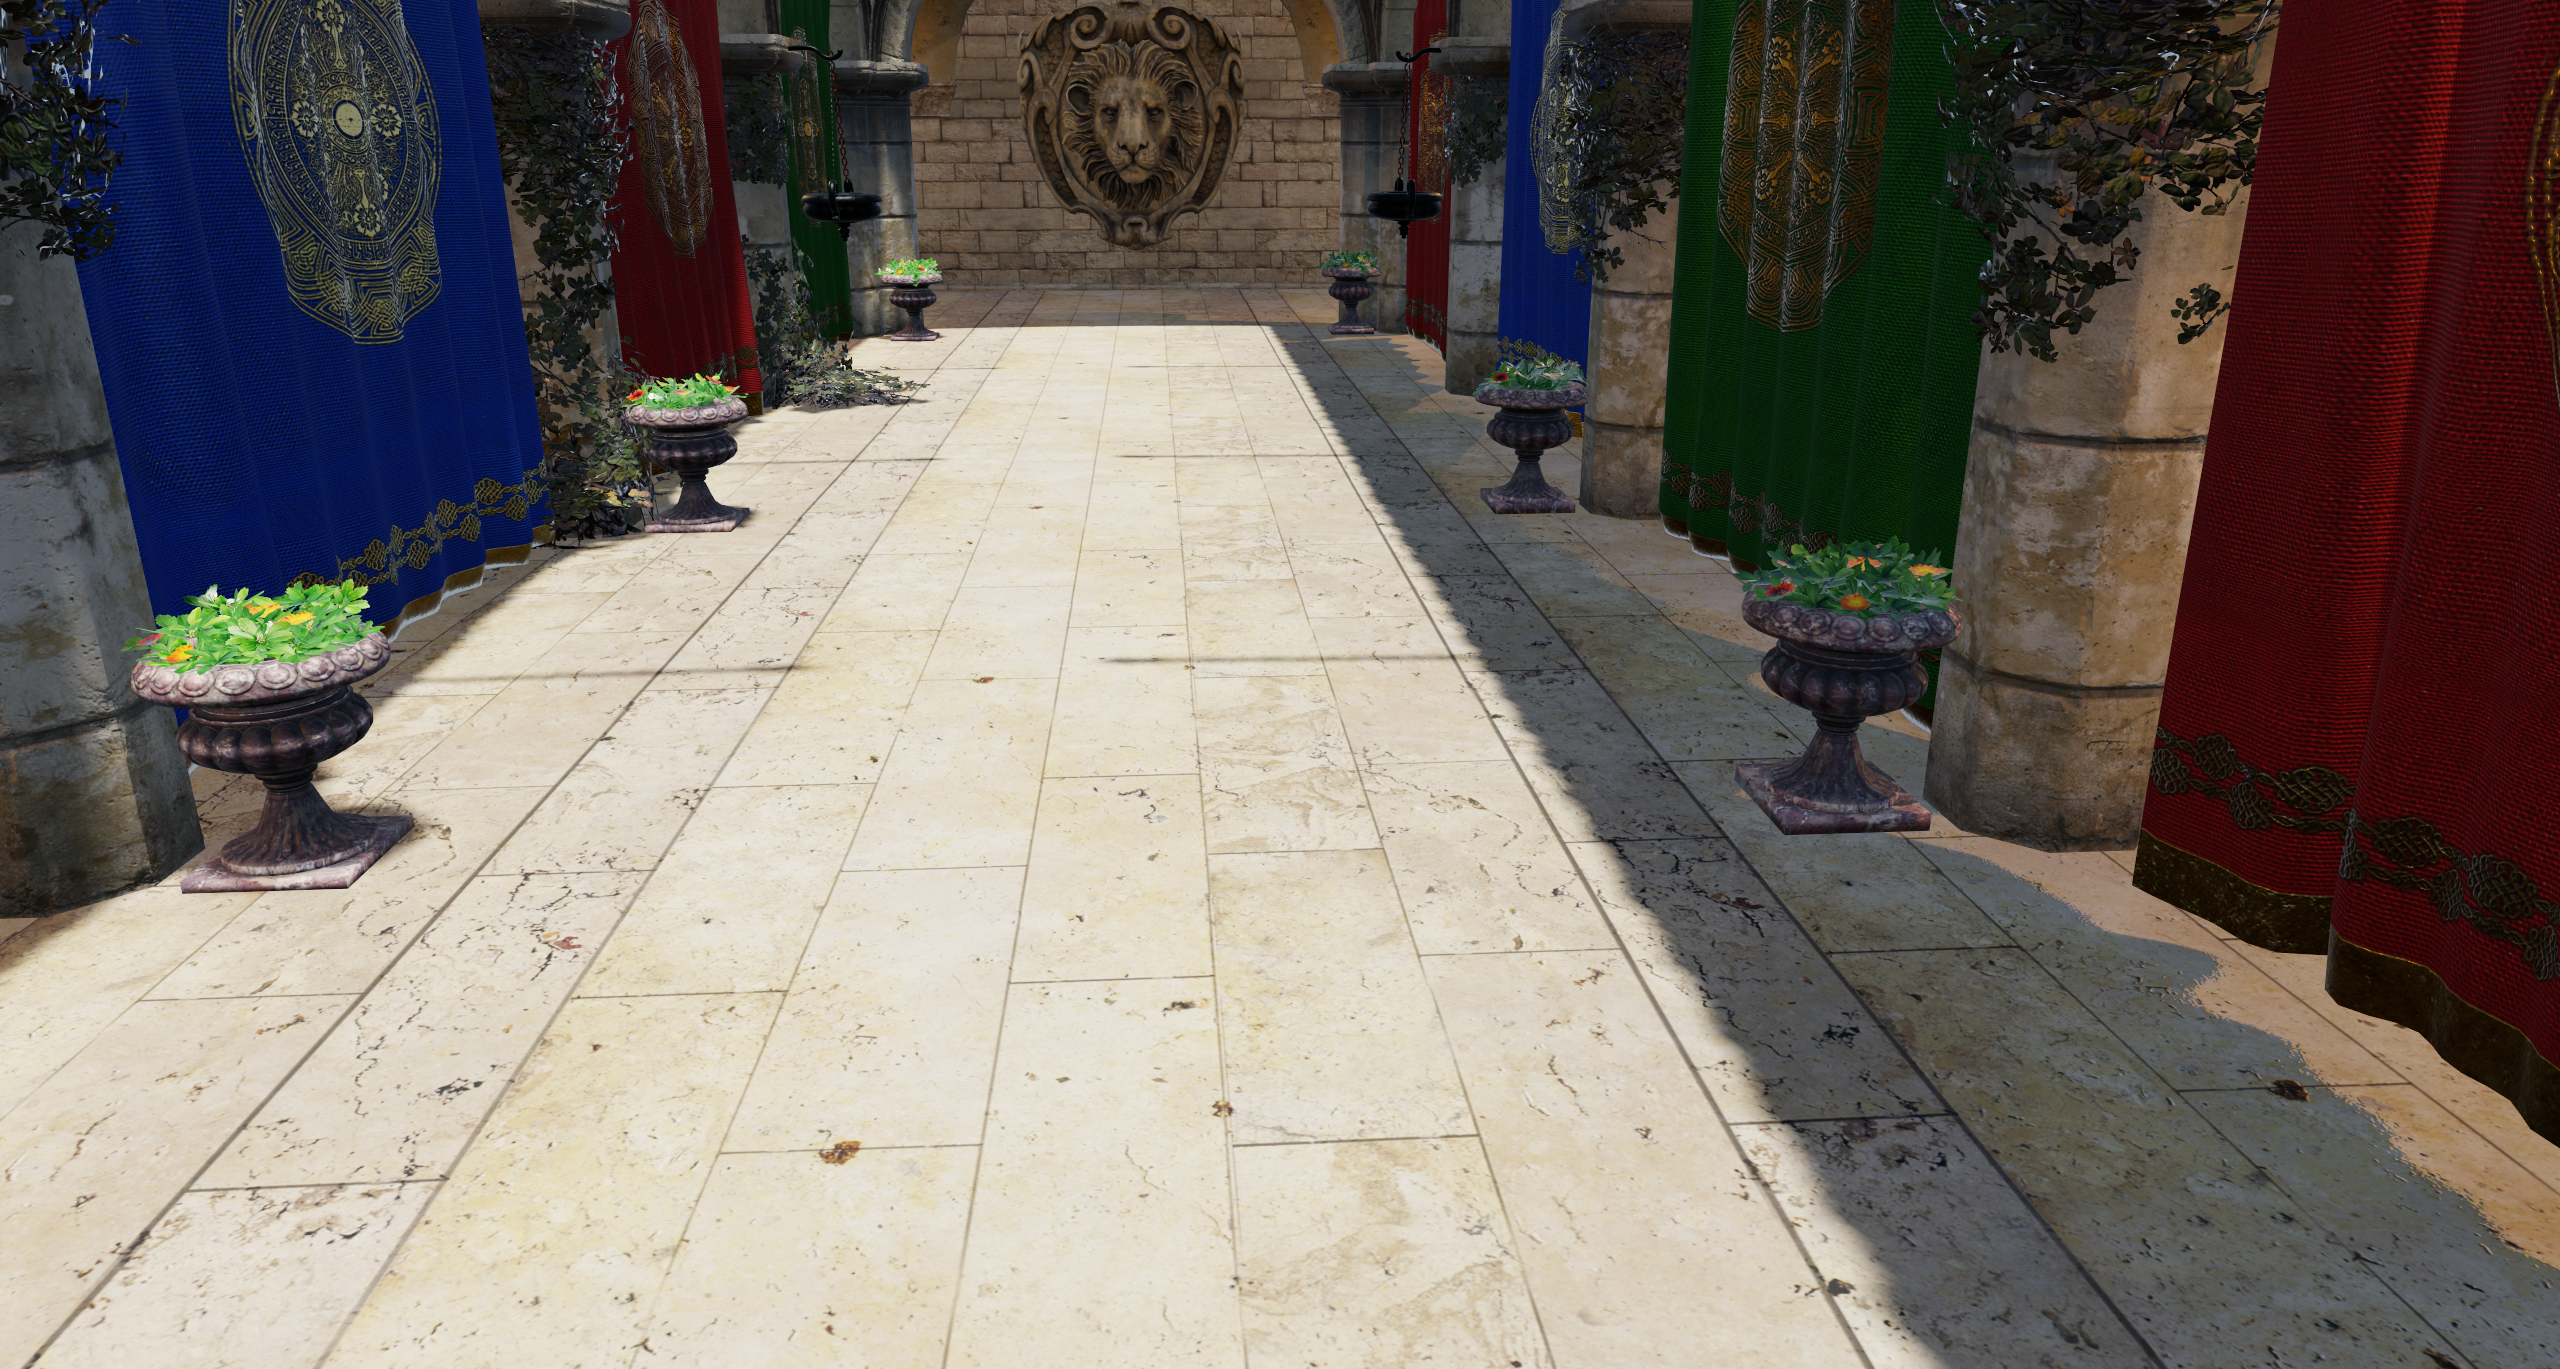
\includegraphics[width=\linewidth]{figures/shadow_map.png}\\{\small shadow mapa (raster)}
\end{minipage}\hfill
\begin{minipage}{0.48\textwidth}\centering
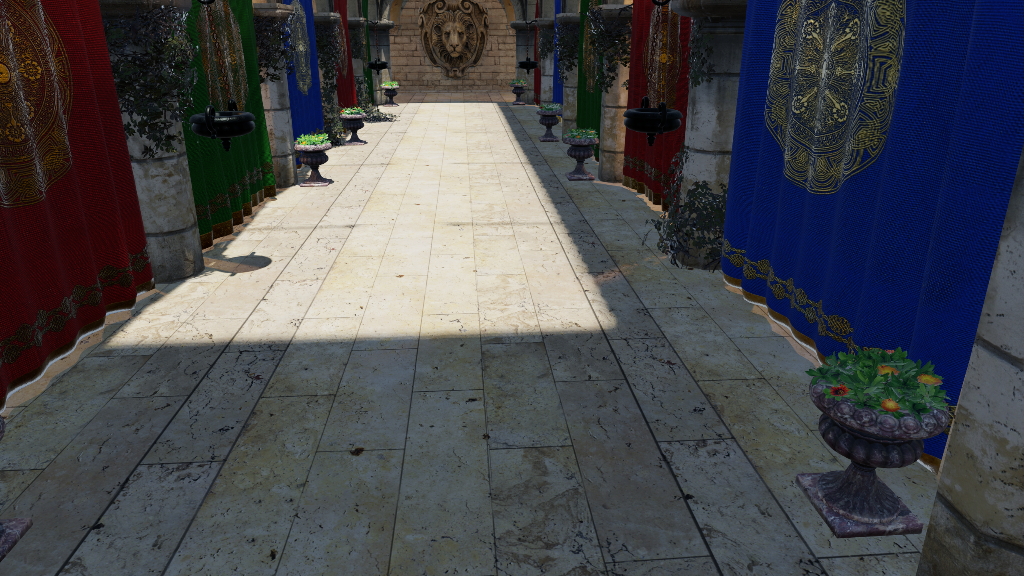
\includegraphics[width=\linewidth]{figures/shadow_rt.png}\\{\small senke pra\'cenjem zraka}
\end{minipage}
\caption[Shadow mapa naspram senki pra\'cenjem zraka]{Ista poza i isto svetlo, \texttt{render.shadows.mode} 1 naspram 2. Urne na osun\v{c}anom podu su mesto na koje treba gledati: rasterska mapa ima kona\v{c}nu rezoluciju i depth bias, pa se njihove kontaktne senke odvajaju od podno\v{z}ja i razmazuju, dok ih pra\'cena verzija usidrava uz pravu geometriju. Snimci su deterministi\v{c}ki (dva uzastopna snimka jedne konfiguracije su bit-identi\v{c}na), pa je svaka razlika izme\dj{}u panela stvarna.}
\label{fig:shadow-vs-map}
\end{figure}


\needspace{22\baselineskip}
\begin{lstlisting}[caption={Inline ray query test vidljivosti za senku (HLSL).}, label={lst:shadow}]
RayQuery<RAY_FLAG_ACCEPT_FIRST_HIT_AND_END_SEARCH> q;
RayDesc ray;
ray.Origin    = positionWS + Ng * 0.02 + L * 0.01;
ray.Direction = L;
ray.TMin      = 0.0;
ray.TMax      = distanceToLight - 0.05;   // sun: effectively infinite
q.TraceRayInline(SceneTLAS, RAY_FLAG_NONE, 0xFF, ray);
while (q.Proceed())                       // alpha-test cutout candidates
{
    if (q.CandidateType() == CANDIDATE_NON_OPAQUE_TRIANGLE &&
        RTCommitCandidate(tableAddr, q.CandidateInstanceID(),
                          q.CandidatePrimitiveIndex(),
                          q.CandidateTriangleBarycentrics(), LinearSampler))
    {
        q.CommitNonOpaqueTriangleHit();
    }
}
bool shadowed = (q.CommittedStatus() == COMMITTED_TRIANGLE_HIT);
\end{lstlisting}

Preko CVar-a \texttt{render.shadow.soft} izlo\v{z}ena su dva nivoa kvaliteta. Tvrda putanja baca jedan zrak pravo ka svetlu, dok meka baca \texttt{SHADOW_RAY_COUNT = 2} zraka koji uzorkuju, uniformno po prostornom uglu, konus pod kojim izvor vidi osen\v{c}ena ta\v{c}ka (Slika~\ref{fig:shadow}), usrednjavaju\'ci pogotke u faktor penumbre u $[0,1]$. Poluugao prati izvor: polovina ugaonog pre\v{c}nika \texttt{render.shadow.sun\_angle\_deg} za sunce i $\arcsin(r/d)$ za lokalno svetlo polupre\v{c}nika \texttt{render.shadow.source\_radius} na rastojanju $d$, pa fizi\v{c}ki ve\'ci ili bli\v{z}i izvor daje mek\v{s}u ivicu. Uzorkovanje prostornog ugla umesto diska u tangentnoj ravni \v{c}ini da se penumbra u realnom vremenu sla\v{z}e sa next-event estimation-om path tracer-a pri bilo kojoj \v{s}irini konusa, a ne samo u granici malih uglova gde se dve parametrizacije poklapaju. \texttt{SHADOW_RAY_COUNT} je konstanta vremena kompajliranja, klasa cene, a ne podesivo dugme.

Pravci dolaze iz spatiotemporal blue noise-a \cite{wolfe2022stbn}, po dve dekorelisane dimenzije po svetlu, pa dvouzorkovnu penumbru raspore\dj{}uju po frejmovima da bi je temporalni akumulator razre\v{s}io (Odeljci~\ref{sec:denoising} i \ref{sec:taa}). Redosled je va\v{z}an iz dva razloga koje slika jednog frejma ne mo\v{z}e da poka\v{z}e: he\v{s} ponovo ba\v{c}en svakog frejma je beo u vremenu i akumulatoru ne ostavlja ni\v{s}ta \v{s}to bi usrednjio, a izvo\dj{}enje obe koordinate konusa iz jednog skalara uru\v{s}ava konus u krivu. Dimenzije po svetlu tako\dj{}e dekoreli\v{s}u svetla me\dj{}usobno, pa im gre\v{s}ka opada sa brojem svetala umesto da se poja\v{c}ava. Cena je \(+0.088\) ms na prolazu Forward, ispod praga materijalnosti iz Odeljka~\ref{sec:cena}.

\begin{figure}[tbp]
\centering
\begin{tikzpicture}[>={Stealth[]}]
  \draw[thick] (-2.6,0) -- (2.6,0);                      % surface
  % light-source disk (perpendicular to L), drawn as a circle
  \draw[fill=black!8] (2.7,2.4) circle (0.45);
  \node[font=\scriptsize, align=center] at (2.7,3.25) {izvor\\(polupre\v{c}nik $r$)};
  % direction to the light centre
  \draw[dashed] (0,0) -- (2.7,2.4);
  \node[font=\scriptsize] at (1.55,1.05) {$L$};
  % sample rays fanning to distinct points across the disk
  \draw[->, black!65] (0,0) -- (2.72,2.83);
  \draw[->, black!65] (0,0) -- (3.08,2.22);
  \draw[->, black!65] (0,0) -- (2.36,2.06);
  \draw[<->, black!45] (2.62,2.72) arc (46:38:3.6);
  \node[font=\scriptsize, black!55] at (3.02,2.52) {$\theta/2$};
  \fill (0,0) circle (1.7pt) node[below=3pt] {$P$};
\end{tikzpicture}
\caption[Uzorkovanje konusa meke senke]{Meke senke: iz ta\v{c}ke $P$ zraci se uzorkuju uniformno po prostornom uglu unutar konusa pod kojim izvor vidi oko pravca $L$, sa poluuglom $\theta/2$ odre\dj{}enim polupre\v{c}nikom izvora $r$ i rastojanjem. Udeo neblokiranih zraka daje penumbru.}
\label{fig:shadow}
\end{figure}

\v{S}irina penumbre je $2H\tan(\theta/2)$ po rastojanju okludera do prijemnika $H$ i ugaonoj veli\v{c}ini izvora $\theta$, zbog \v{c}ega Slika~\ref{fig:shadow-hs} kadrira osun\v{c}anu traku poda: sunce je jedino svetlo ovde sa udaljenim okluderom, dok se \v{c}etiri uklju\v{c}ene baklje nalaze na par jedinica od zidova koje osvetljavaju. \v{C}ak i tu pravi ugaoni pre\v{c}nik daje oko 36 piksela na snimku \v{s}irine 2560, pa ga slika preuveli\v{c}ava i to navodi.

Pogon suncem umesto preko \texttt{render.shadow.source\_radius} je namerna odluka, iz razloga koji je ujedno i ograni\v{c}enje. Uzorci konusa koji padaju ispod horizonta normale \v{s}ejdiranja preska\v{c}u se, a prosek se i dalje deli punim brojem uzoraka, \v{s}to je samo po sebi ispravno (njihovo ra\v{c}unanje kao osvetljenih je curenje koje next-event estimation u path tracer-u odbacuje), iako zna\v{c}i da \v{s}iri konus sistematski zatamnjuje povr\v{s}ine pod o\v{s}trim uglom. Pri polupre\v{c}niku od 1.5 jedinica to zatamnjenje \v{c}ini oko tri \v{c}etvrtine razlike me\dj{}u frejmovima i gu\v{s}i penumbru koju je trebalo da poka\v{z}e. Skoro vertikalno sunce to izbegava, jer poga\dj{}a pod tamo gde ni\v{s}ta nije odba\v{c}eno zbog horizonta.

\begin{figure}[tbp]
\centering
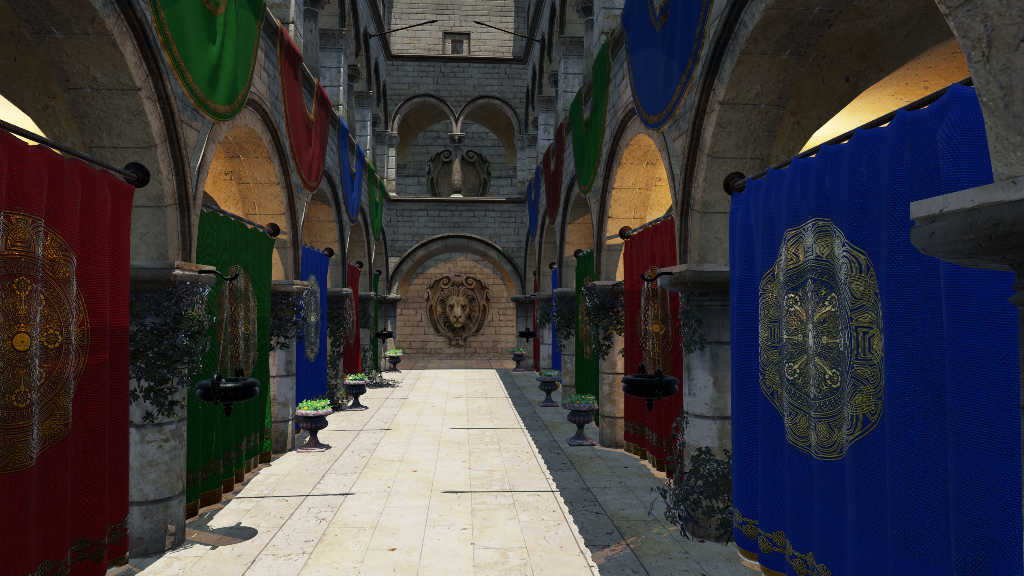
\includegraphics[width=0.48\textwidth]{figures/shadow_hard.png}\hfill%
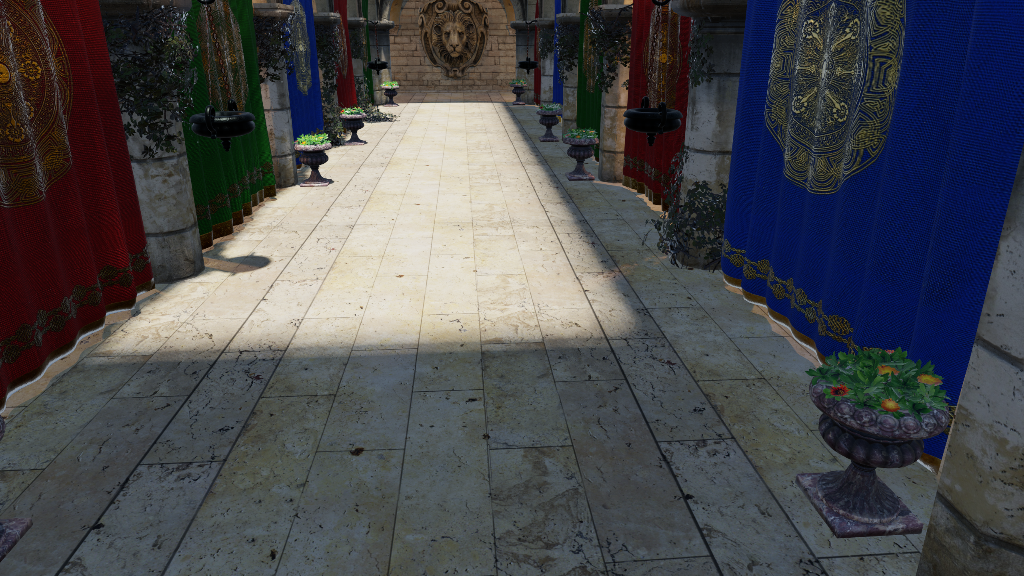
\includegraphics[width=0.48\textwidth]{figures/shadow_soft.png}
\caption[Tvrde naspram mekih senki pra\'cenjem zraka]{Tvrde (levo) naspram mekih (desno) senki pra\'cenjem zraka na osun\v{c}anoj traci poda, koje baca ivica krovnog svetlarnika oko 10.4 jedinica iznad nje: jedina razlika je \texttt{render.shadow.soft}. Ugaoni pre\v{c}nik sunca podignut je na $3^\circ$, oko \v{s}est puta fizi\v{c}kih $0.53^\circ$, jer je pri pravoj vrednosti penumbra u\v{z}a nego \v{s}to \v{s}tampa mo\v{z}e da razre\v{s}i. Treba \v{c}itati \v{s}irinu prelaza, a ne njegovu \v{c}isto\'cu: tvrda ivica nosi i detalj siluete ivice svetlarnika, koji penumbra usrednjava, pa se paneli razlikuju i u o\v{s}trini i u izlomljenosti istovremeno, a samo prva je predmet. Penumbra ovde ima otprilike konstantnu \v{s}irinu jer je baca jedan okluder na jednoj visini. \v{S}irenje sa rastojanjem okludera, re\v{c}itiji potpis povr\v{s}inskog izvora, zahtevalo bi senku koja putuje, a sa suncem na $80^\circ$ iznad horizonta ni\v{s}ta u ovoj sceni takvu ne baca.}
\label{fig:shadow-hs}
\end{figure}

\paragraph{Stohasti\v{c}ka alternativa.} Pra\'cenje svakog svetla u svakom pikselu je ta\v{c}no, ali raste linearno sa brojem svetala, \v{s}to ne pre\v{z}ivljava scenu osvetljenu stotinama izvora. Engine zato implementira drugu strategiju, uklju\v{c}enu preko \texttt{render.shadows.stochastic} i podrazumevano isklju\v{c}enu, prema MegaLights pristupu \cite{epic_megalights}: svaki piksel uzima \texttt{render.shadows.rays} nezavisnih uzoraka (ovaj CVar pokre\'ce samo ovu putanju, a ne inline gore, \v{c}iji je broj zraka konstanta vremena kompajliranja), a svaki uzorak zasebno koristi resampled importance sampling \cite{talbot2005ris} da izabere \emph{jedno} svetlo sa verovatno\'com proporcionalnom njegovom nezasen\v{c}enom doprinosu i prati jedan zrak ka njemu. Usrednjavanje uzoraka daje jedan agregatni odnos vidljivosti, pa cenu odre\dj{}uje broj uzoraka, a ne broj svetala. Procena je nepristrasna, ali izuzetno \v{s}umovita, jer uzorci jednog piksela ne govore ni\v{s}ta o tome koja je svetla izvukao njegov sused, pa ova putanja nu\v{z}no radi kao poseban lanac u polovini rezolucije, \texttt{RTShadow} $\rightarrow$ \texttt{ShadowTemporal} $\rightarrow$ \texttt{ShadowDenoise0..2} $\rightarrow$ \texttt{ShadowUpsample}, koji ponovo koristi zajedni\v{c}ki denoiser, uz paralelni lanac demodulisanog spekulara za \v{c}lan spekularne okluzije. Ti prolazi nose sopstvene GPU timestamp opsege, koje Odeljak~\ref{sec:cena} obra\v{c}unava odvojeno od forward prolaza. Njena cena je konstantna po broju svetala, \v{s}to je ceo smisao: inline putanja pobe\dj{}uje za mali broj svetala, a gubi za mnogo. Odeljak~\ref{sec:analiza-shadow-strategy} meri ta\v{c}ku preseka na ovoj sceni, a debug prikazi izla\v{z}u agregatni bafer vidljivosti pre i posle filtriranja (Slika~\ref{fig:shadow-denoise-ab}), gde toliko malo uzoraka po pikselu ostavlja sirov odnos skoro binarnim \v{s}umom.

Podrazumevano je isklju\v{c}ena, a razlog je kompromis koji rekonstrukcija trenutno ne mo\v{z}e da razre\v{s}i. Njena procena po frejmu je bimodalna, ili nula ili redak svetao pik, zavisno od toga koje je svetlo piksel ponovo uzorkovao, a clamp boje u susedstvu, koji uklanja duhove na pokretnim ivicama iz GI i refleksija, pogre\v{s}an je za signal takvog oblika: gde se dva svetla preklapaju, lokalni opseg je uzak i taman, pa clamp dr\v{z}i akumuliranu istoriju dole i ostavlja crni \v{s}av izme\dj{}u dva svetla koji nikakvo filtriranje ne popunjava. Isklju\v{c}ivanje clamp-a tu, \v{s}to je isporu\v{c}eno pode\v{s}avanje, uklanja \v{s}av i vra\'ca razmazivanje pri kretanju kamere koje je clamp trebalo da spre\v{c}i. Oba izbora ostavljaju vidljiv defekt, pa inline ostaje podr\v{z}ana putanja.

Merenja se ne protive ni\v{c}emu od toga, a jedno od njih aktivno pokazuje pogre\v{s}nim smerom. Na ruti sa kretanjem stohasti\v{c}ka putanja je temporalno stabilnija od dve, tFLIP \mMegalightsTflip{} naspram \mRtShadowTflip{} inline-a, a Odeljak~\ref{sec:analiza-shadow-strategy} nalazi da je jeftinija od dve na RX 9070 XT. Ocenu stabilnosti treba \v{c}itati uz razmazivanje, a ne protiv njega: mera toga koliko se rezultat malo menja izme\dj{}u frejmova ne mo\v{z}e da razdvoji stabilno od razmazanog, \v{s}to Odeljak~\ref{sec:motion} obra\dj{}uje sa ovim parom kao radnim primerom. \v{S}av izmi\v{c}e merenju iz prozai\v{c}nijeg razloga, jer ruta nikad ne kadrira osvetljene bo\v{c}ne prolaze gde se dve baklje preklapaju. Podrazumevana vrednost je dakle postavljena uprkos metrikama, a ne prema njima, \v{s}to vredi otvoreno re\'ci u radu koji se ina\v{c}e oslanja na merenje.

\begin{figure}[tbp]
\centering
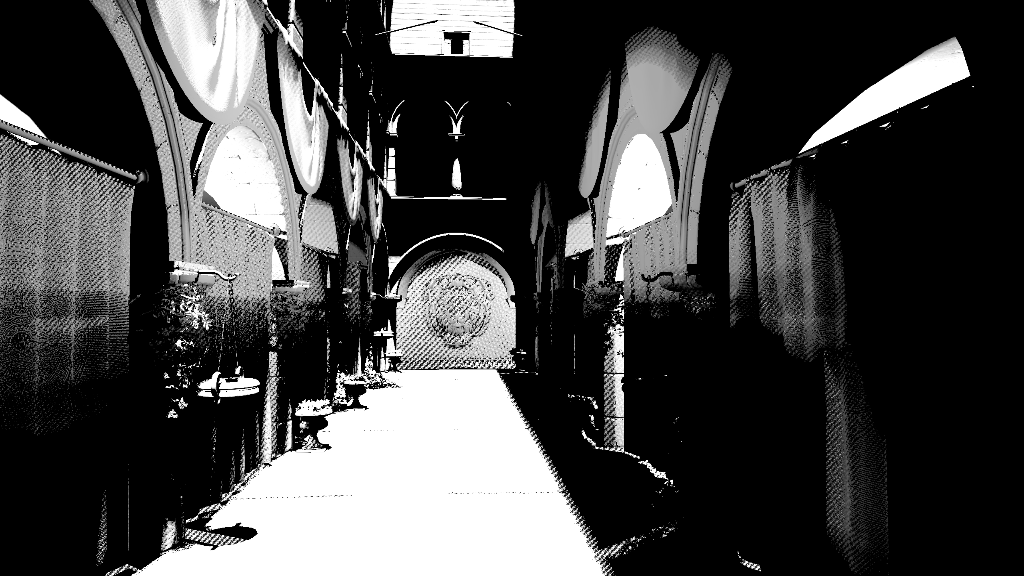
\includegraphics[width=0.48\textwidth]{figures/dbg_shadow_raw.png}\hfill%
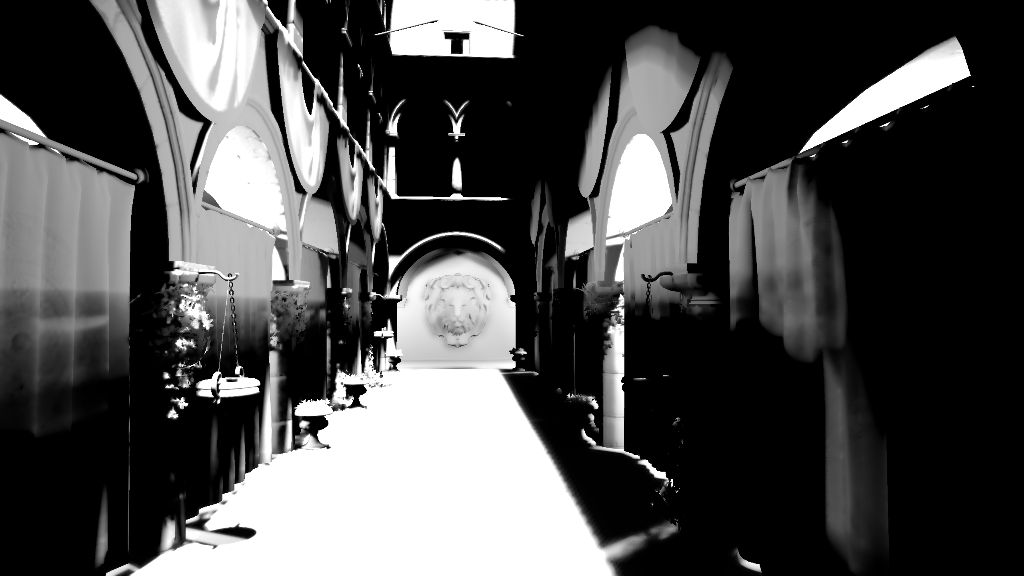
\includegraphics[width=0.48\textwidth]{figures/dbg_shadow_denoised.png}
\caption[Stohasti\v{c}ka vidljivost pre i posle denoising-a]{Stohasti\v{c}ki agregatni odnos vidljivosti pre (levo) i posle (desno) temporalne akumulacije i a-trous filtera (\texttt{render.debugview} 8 i 9). Belo je potpuno osvetljeno, crno potpuno u senci. Levi panel pokazuje koliko je sirov odnos po pikselu skoro binaran pri ovom broju uzoraka.}
\label{fig:shadow-denoise-ab}
\end{figure}

\subsection{Ambijentalna okluzija (AO)}

Ambijentalna okluzija je compute prolaz (\texttt{AO.comp.hlsl}) u polovini rezolucije. Svaki piksel rekonstrui\v{s}e svetsku poziciju iz G-bafera dubine i baca \texttt{render.ao.rays} kratkih zraka (podrazumevano 2, ograni\v{c}eno na $[1,16]$) po hemisferi sa kosinusnom te\v{z}inom oko geometrijske normale, rotiranoj po pikselu interleaved gradient noise-om, koriste\'ci isti \texttt{ACCEPT_FIRST_HIT_AND_END_SEARCH} obilazak vidljivosti kao senke. Zraci su ograni\v{c}eni na \texttt{render.ao.radius}, a pogodak doprinosi \texttt{1 - saturate(t / AORadius)}, pa bli\v{z}i okluderi zatamnjuju vi\v{s}e, a rezultat se skalira sa \texttt{render.ao.intensity} (Listing~\ref{lst:ao}). Slika~\ref{fig:ao-composited} pokazuje \v{s}ta to doprinosi gotovoj slici, a Slika~\ref{fig:ssvsrt-ao} pokazuje sam \v{c}lan naspram screen-space alternative.

\begin{figure}[tbp]
\centering
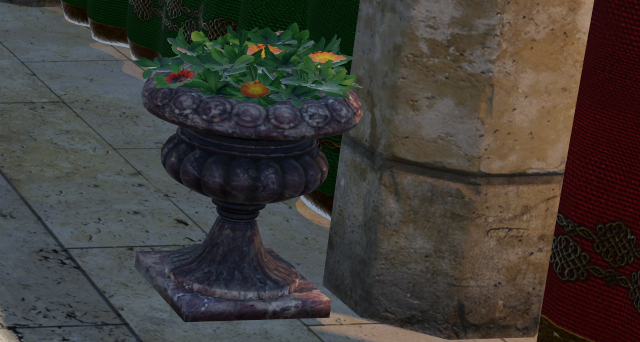
\includegraphics[width=0.485\textwidth]{figures/ao_off.png}\hfill
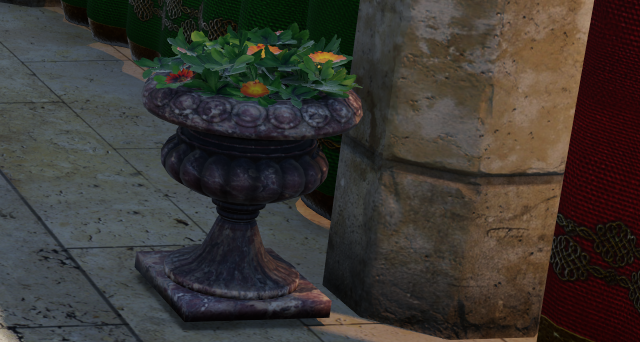
\includegraphics[width=0.485\textwidth]{figures/ao_on.png}
\caption[Ambijentalna okluzija u kompozitnom frejmu]{Ambijentalna okluzija isklju\v{c}ena (levo) i uklju\v{c}ena (desno), u gotovom frejmu a ne u AO baferu. Ovo je ise\v{c}ak, namerno: okluzija nastaje tamo gde geometrija obuhvata geometriju, pa je preko celog frejma efekat vredan 2.4 nivoa od 255 i neise\v{c}en par bi se \v{s}tampao kao dve identi\v{c}ne slike. Ovde je 6.2, a dobija se postolje usa\dj{}eno u pod umesto da lebdi nad njim, dubina izme\dj{}u listova i stub koji dodiruje tlo umesto da kroz njega prolazi. Odeljak~\ref{sec:poredjenje} je isto zapa\v{z}anje kao broj: AO ostavlja netaknuto pet \v{s}estina ovog frejma.}
\label{fig:ao-composited}
\end{figure}


\needspace{17\baselineskip}
\begin{lstlisting}[caption={Uzorkovanje hemisfere za AO (HLSL, reprezentativan ise\v{c}ak).}, label={lst:ao}]
float occlusion = 0.0;
for (uint k = 0; k < RayCount; ++k)
{
    float3 dir = CosineHemisphere(k, RayCount, ign, N); // cosine-weighted, IGN-rotated around N
    RayQuery<RAY_FLAG_ACCEPT_FIRST_HIT_AND_END_SEARCH> q;
    RayDesc ray = MakeRay(positionWS + N * 0.02, dir, 0.0, AORadius);
    q.TraceRayInline(SceneTLAS, RAY_FLAG_NONE, 0xFF, ray);
    while (q.Proceed()) { /* alpha-test cutout candidates, as in Listing 3.1 */ }
    if (q.CommittedStatus() == COMMITTED_TRIANGLE_HIT)
        occlusion += 1.0 - saturate(q.CommittedRayT() / AORadius);
}
occlusion = 1.0 - occlusion / RayCount;
\end{lstlisting}

Prolaz pi\v{s}e \texttt{float4(ao, ao, ao, meanHitT)}, pri \v{c}emu alfa kanal nosi srednje rastojanje do okludera. Taj alfa napaja \v{c}lan zaustavljanja ivica vo\dj{}en rastojanjem pogotka u denoiser-u (Odeljak~\ref{sec:denoising}), istu ideju koju NVIDIA-in ReBLUR denoiser \cite{nvidia_nrd} koristi da skalira prostorni filter prema tome koliko je okluder bio daleko. \v{C}lan je implementiran, ali podrazumevano isklju\v{c}en na svakom signalu, uklju\v{c}uju\'ci AO: pri dva zraka po pikselu rastojanje pogotka je previ\v{s}e \v{s}umovito da bi usmeravalo filter, a pogre\v{s}no usmeravanje je gore od nikakvog. Rezultat u polovini rezolucije se denoisuje i bilateralno upsample-uje pre nego \v{s}to ga forward prolaz pomno\v{z}i u ambijentalni \v{c}lan (Slika~\ref{fig:ao}).

\begin{figure}[tbp]
\centering
\begin{tikzpicture}[>={Stealth[]}]
  \draw[thick] (-2.7,0) -- (2.7,0);
  \draw[dashed] (-1.9,0) arc (180:0:1.9);
  \draw[->, thick] (0,0) -- (0,2.25) node[above] {$N$};
  \foreach \a in {30,60,90,120,150} \draw[->, black!60] (0,0) -- (\a:1.9);
  \draw[fill=black!12] (0.85,0.55) rectangle (1.3,1.25);
  \draw[thin] (1.3,1.1) -- (2.05,1.6);
  \node[font=\scriptsize, anchor=west] at (2.05,1.6) {okluder};
  \fill (0,0) circle (1.7pt) node[below=3pt] {$P$};
\end{tikzpicture}
\caption[Uzorkovanje hemisfere za ambijentalnu okluziju]{Uzorkovanje hemisfere za AO: iz ta\v{c}ke $P$ baca se nekoliko kratkih zraka po hemisferi oko normale $N$. Udeo koji poga\dj{}a geometriju unutar zadatog polupre\v{c}nika daje okluziju.}
\label{fig:ao}
\end{figure}

\subsection{Refleksije}

Refleksije su compute prolaz (\texttt{Reflection.comp.hlsl}) u punoj rezoluciji, za razliku od GI i AO gather-a u polovini rezolucije, jer detalj refleksije zavisi od pogleda i ne podnosi zamu\'cenje koje unosi pra\'cenje u polovini rezolucije plus upsample. Pikseli \v{c}ija je hrapavost jednaka ili ve\'ca od \texttt{render.reflections.max\_roughness} (podrazumevano 0.8) preska\v{c}u se i zadr\v{z}avaju spekular iz prefiltriranog cube-a, pa udeo frejma koji se prati zavisi od me\v{s}avine materijala u sceni. Svaki preostali piksel rekonstrui\v{s}e svetsku poziciju i reflektuje vektor pogleda oko normale \v{s}ejdiranja sa normal mapom (\v{c}ita se iz zasebnog G-bafera normala \v{s}ejdiranja, a ne geometrijske normale, pa se normal mape ispravno ogledaju; pe\v{c}ene normal mape su BC5, koji \v{c}uva samo X i Y, pa Z rekonstrui\v{s}e \texttt{NormalEncode.hlsli}, a path tracer dekodira kroz istu funkciju). Treba mu najbli\v{z}i pogodak, pa za razliku od upita vidljivosti koristi obi\v{c}an \texttt{RayQuery<RAY_FLAG_NONE>} i izvr\v{s}ava obilazak do kraja.

Sjajne refleksije se aproksimiraju pomeranjem svakog zraka unutar konusa \v{c}iji poluugao raste sa hrapavo\v{s}\'cu povr\v{s}ine (\texttt{roughness * ReflConeScale}), usrednjeno preko \texttt{render.reflections.rays} (podrazumevano 1), dok se ogledalska povr\v{s}ina (\texttt{roughness == 0}) svodi na jedan o\v{s}tar zrak. Pogoci se \v{s}ejdiraju preko \texttt{ShadeSurfaceHit} (sun\v{c}evo osvetljenje sa sopstvenim zrakom senke, emisivni \v{c}lan pogo\dj{}ene povr\v{s}ine, image-based ambijent), a proma\v{s}aj uzorkuje prefiltrirani cube neba. Za razliku od GI prolaza ispod, refleksije ne uzorkuju lokalna ta\v{c}kasta i spot svetla scene u pogotku. Isti importance-sampled estimator lokalnih svetala izmeren je i ovde i nije pomerio nijednu metriku kvaliteta za dvostruku cenu GI strane, pa je potpuno izba\v{c}en iz ovog prolaza pri kompajliranju umesto da je ostavljen iza isklju\v{c}ene zastavice, po istom standardu dokaza pre svega koji podrazumevano isklju\v{c}uje gore navedeni vodi\v{c} rastojanja pogotka. Prolaz pi\v{s}e sirovu reflektovanu radijansu plus rastojanje pogotka, dok se Fresnelov \v{c}lan, te\v{z}injenje BRDF-om i \texttt{render.reflections.intensity} primenjuju naknadno u forward prolazu (Slika~\ref{fig:refl}).

\begin{figure}[tbp]
\centering
\begin{tikzpicture}[>={Stealth[]}]
  \draw[thick] (-2.7,0) -- (2.7,0);
  \draw[->, thick] (0,0) -- (0,2.2) node[above] {$N$};
  \draw[->, black!55] (-2.05,2.05) -- (0,0); \node[font=\scriptsize] at (-1.55,1.35) {$V$};
  \foreach \a in {50,62,74} \draw[->, black!65] (0,0) -- (\a:2.15);
  \draw[dashed] (0,0) -- (62:2.3) node[above right, font=\scriptsize] {$R$};
  \node[font=\scriptsize, align=center] at (2.0,1.05) {konus\\(hrapavost)};
  \fill (0,0) circle (1.7pt) node[below=3pt] {$P$};
\end{tikzpicture}
\caption[Reflektovani pravac i konus hrapavosti]{Refleksije: reflektovani pravac $R$ vektora pogleda $V$ oko normale $N$. Glatka povr\v{s}ina daje jedan o\v{s}tar zrak, a gruba uzorkuje konus oko $R$.}
\label{fig:refl}
\end{figure}

Slika~\ref{fig:refl-onoff} pokazuje doprinos prolaza. Variranje \texttt{render.reflections.cone\_scale} od 0 (\v{c}ist ogledalski zrak) do 3 menja gotov frejm u proseku samo za 0.16 nivoa od 255, preko \v{s}est isprobanih poza kamere, dok isto A/B, izmereno na baferu refleksija pre kompozicije, pomera 43.7 nivoa i spu\v{s}ta visokofrekventnu energiju bafera sa \hfConeSharp{} na \hfConeGlossy{}, \v{s}to je 275 puta vi\v{s}e signala nego \v{s}to pokazuje kompozitno pore\dj{}enje. Uzrok je to \v{s}to je refleksija mali aditivni \v{c}lan pored direktnog osvetljenja, pa ga kompozitna slika krije: \v{c}lan koji je mali u kona\v{c}noj slici i dalje mo\v{z}e biti ceo sadr\v{z}aj svog me\dj{}ubafera. Slika konusa (Slika~\ref{fig:refl-cone}) stoga koristi izolovani bafer, iz istog razloga iz kog to radi i galerija efekata u Odeljku~\ref{sec:cena}.

\begin{figure}[tbp]
\centering
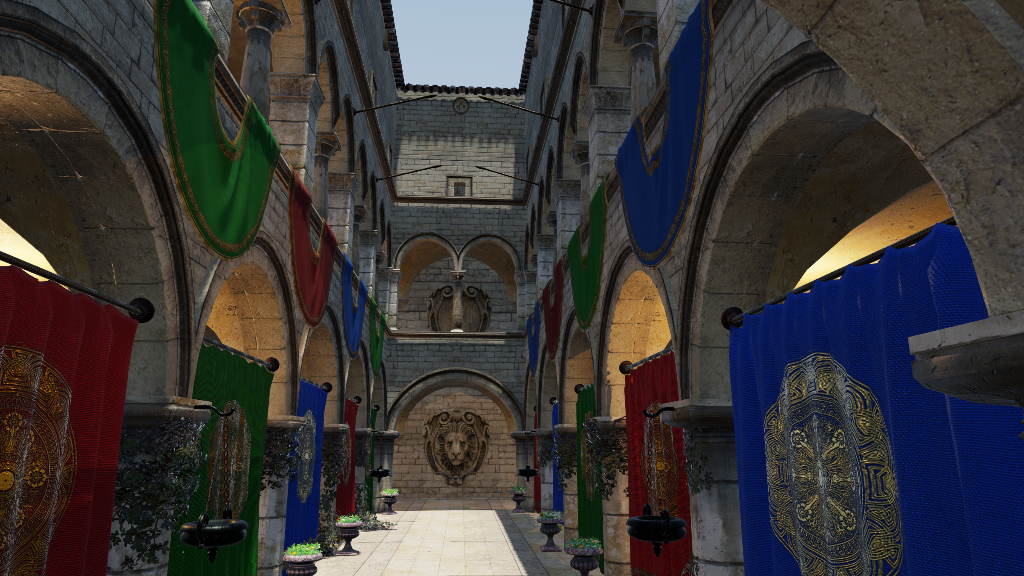
\includegraphics[width=0.48\textwidth]{figures/refl_off.png}\hfill%
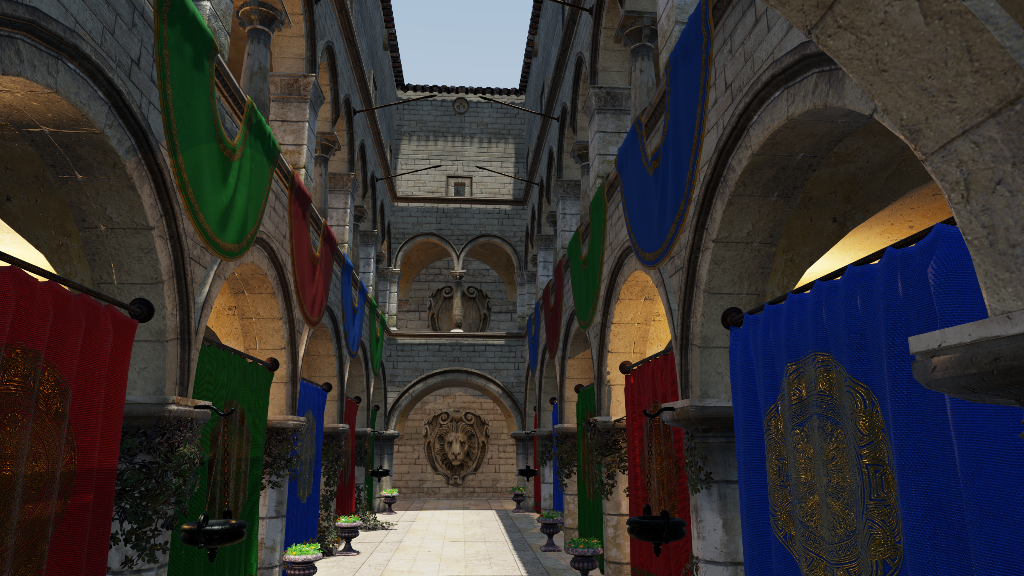
\includegraphics[width=0.48\textwidth]{figures/refl_rt.png}
\caption[Refleksije isklju\v{c}ene naspram refleksija pra\'cenjem zraka]{Bez refleksija (levo) naspram sa njima (desno), ise\v{c}eno na zlatni konac na draperiji pod uglom bliskim klize\'cem, gde je Fresnelov doprinos najve\'ci. Ise\v{c}eno iz istog razloga kao Slika~\ref{fig:ao-composited}: preko celog frejma prolaz vredi 3.3 nivoa od 255, a ovde 11.8. Dodaje se konac koji iz ravne boje prelazi u ne\v{s}to sa metalnim sjajem koji se menja dok se povr\v{s}ina okre\'ce. Vredi re\'ci \v{s}ta ova slika ne mo\v{z}e da poka\v{z}e, jer to ograni\v{c}ava efekat u ovoj sceni, a ne u tehnici: Sponza nema ogledalsku povr\v{s}inu, pa bafer refleksija vra\'ca ne\v{s}to spekulara od skoro svakog materijala, a prepoznatljivu reflektovanu sliku ni od jednog.}
\label{fig:refl-onoff}
\end{figure}

\begin{figure}[tbp]
\centering
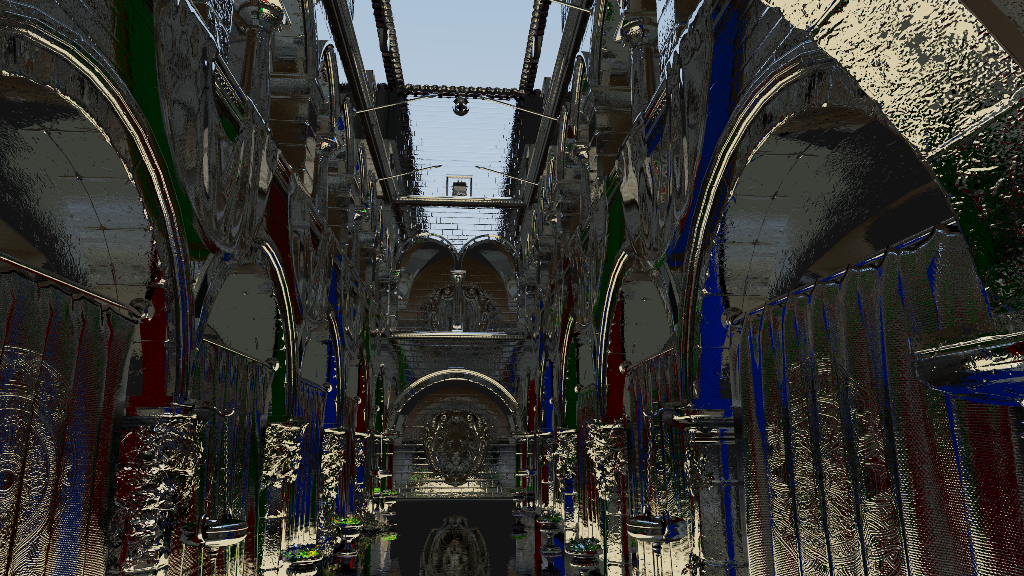
\includegraphics[width=0.48\textwidth]{figures/cone_sharp.png}\hfill%
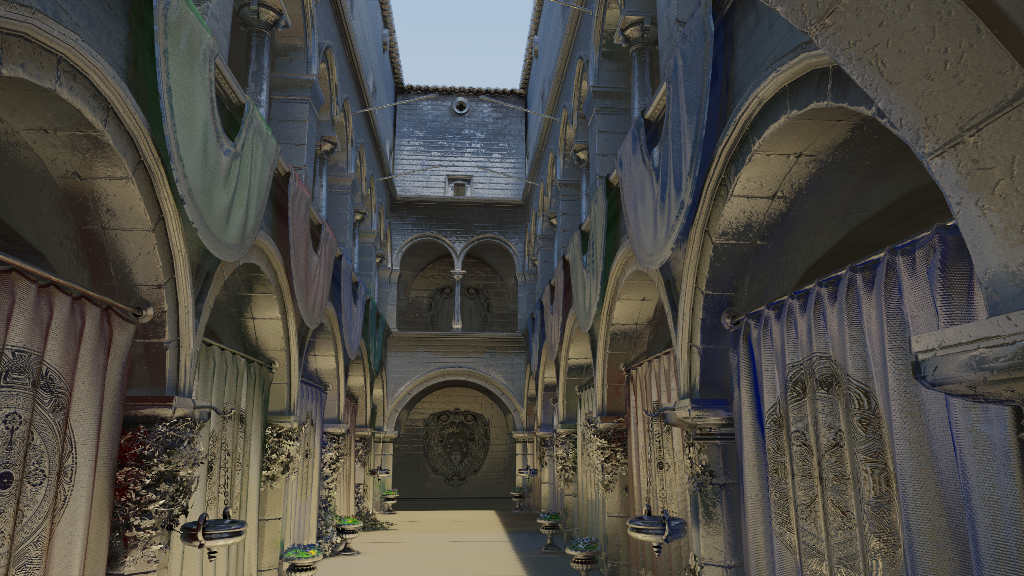
\includegraphics[width=0.48\textwidth]{figures/cone_glossy.png}
\caption[O\v{s}tar naspram sjajnog bafera refleksija]{Reflektovana radijansa pre kompozicije (\texttt{render.debugview} 3): o\v{s}tar ogledalski zrak, \texttt{cone\_scale} 0 (levo), naspram konusa pro\v{s}irenog hrapavo\v{s}\'cu, \texttt{cone\_scale} 3 (desno). Razlika je nevidljiva u gotovoj slici jer je refleksija mali aditivni \v{c}lan pored direktnog osvetljenja, iako je u sopstvenom baferu ceo sadr\v{z}aj.}
\label{fig:refl-cone}
\end{figure}

\subsection{Globalno osvetljenje (GI)}

Globalno osvetljenje je najskuplji efekat: compute prolaz (\texttt{GI.comp.hlsl}) u polovini rezolucije koji ra\v{c}una jedan odskok difuzne indirektne svetlosti. Hemisferu uzorkuje ta\v{c}no kao AO, \texttt{render.gi.rays} zraka (podrazumevano 2) do \texttt{render.gi.range}. Razlika je u onome \v{s}to zrak vra\'ca. Proma\v{s}aj uzorkuje cube neba, a svaki pogodak \v{s}ejdira \texttt{ShadeSurfaceHit}: sunce sa sopstvenim zrakom senke, emisivni \v{c}lan pogo\dj{}ene povr\v{s}ine, image-based ambijentalno punjenje i, kad je \texttt{render.rt.hit_lights} uklju\v{c}eno (podrazumevano), jedno od ta\v{c}kastih i spot svetala scene. To svetlo se bira importance sampling-om proporcionalno svom nezasen\v{c}enom doprinosu u pogotku i potvr\dj{}uje sopstvenim zrakom senke, kao nepristrasan estimator sa jednim uzorkom (isti koji koristi \texttt{RTShadowPass}, u duhu UE5 MegaLights) \v{c}ija je cena konstantna po broju svetala, za razliku od pune next-event estimation sume preko svih svetala, koja bi pomno\v{z}ila bud\v{z}et zraka u svakom sekundarnom pogotku. Ovaj \v{c}lan va\v{z}i samo za GI, a rutina ne prati dalje od ovih zraka senki, pa evaluacija ostaje jedan odskok.

Prolaz daje samo dolaznu iradijansu, bez albeda prijemnika, koji se mno\v{z}i u punoj rezoluciji u forward prolazu. To je konvencija demodulisane iradijanse na koju se oslanjaju i SVGF denoiser i probe sistemi poput DDGI/RTXGI \cite{majercik2019ddgi, nvidia_rtxgi}: filtriranje iradijanse umesto kona\v{c}ne boje spre\v{c}ava da detalj teksture albeda zavara zaustavljanje ivica denoisera. Forward prolaz zatim menja svoj ravni ambijentalni \v{c}lan ovim indirektnim osvetljenjem dobijenim pra\'cenjem zraka, istom zamenom koju prave Lumen i RTXGI \cite{epic_lumen}. Pri dva zraka po pikselu i polovini rezolucije (Slika~\ref{fig:gi}) sirov izlaz je upotrebljiv tek posle temporalnog-plus-prostornog denoise-a iz Odeljka~\ref{sec:denoising}.

\begin{figure}[tbp]
\centering
\begin{tikzpicture}[>={Stealth[]}]
  \draw[thick] (-2.9,0) -- (2.9,0);
  \draw[dashed] (-2.1,0) arc (180:0:2.1);
  \draw[->, thick] (0,0) -- (0,2.45) node[above] {$N$};
  \foreach \a in {35,70,110,145} \draw[->, black!60] (0,0) -- (\a:2.1);
  \foreach \a in {35,70,110,145} \fill[black!30] (\a:2.1) circle (2.4pt);
  \fill (0,0) circle (1.7pt) node[below=3pt] {$P$};
\end{tikzpicture}
\caption[Uzorkovanje hemisfere sa kosinusnom te\v{z}inom za GI]{Globalno osvetljenje: uzorkovanje hemisfere sa kosinusnom te\v{z}inom oko $N$ iz ta\v{c}ke $P$. Svaki zrak koji pogodi geometriju vra\'ca radijansu (jedan odskok).}
\label{fig:gi}
\end{figure}

Slika~\ref{fig:gi-onoff} prikazuje scenu bez globalnog osvetljenja pra\'cenjem zraka i sa njim.

\begin{figure}[tbp]
\centering
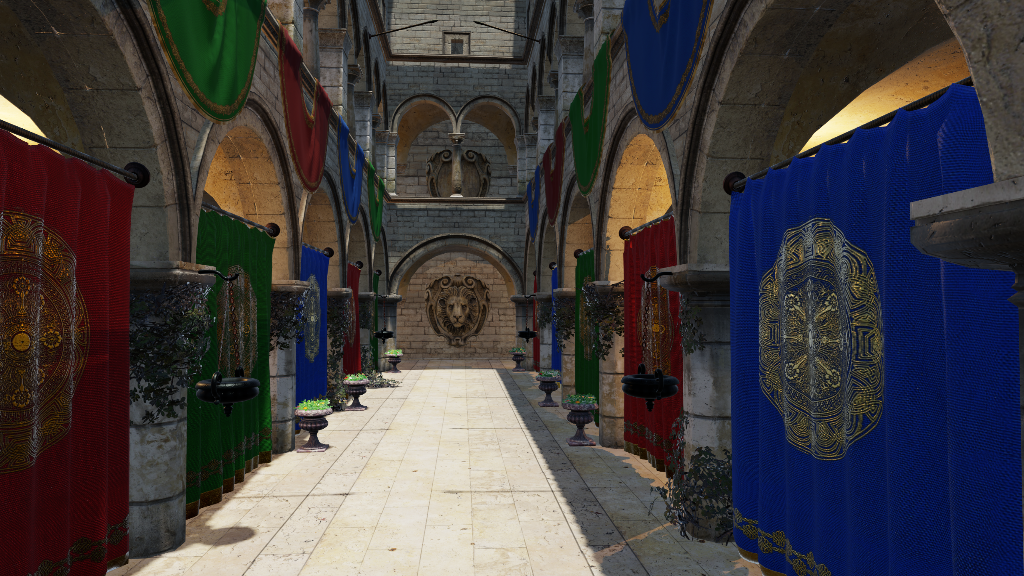
\includegraphics[width=0.82\textwidth]{figures/gi_off.png}

\vspace{6pt}

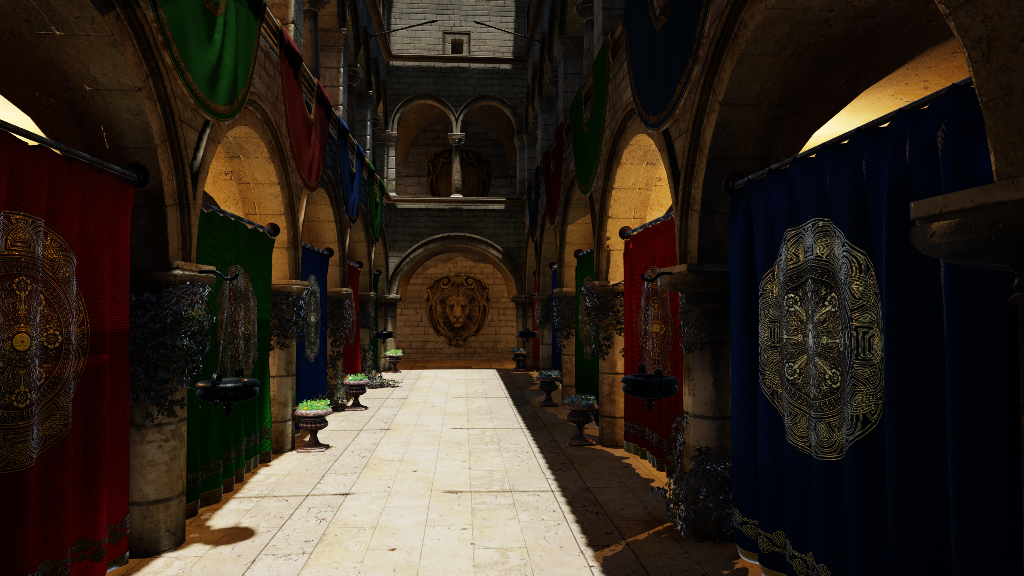
\includegraphics[width=0.82\textwidth]{figures/gi_on.png}
\caption[Scena bez globalnog osvetljenja i sa njim]{Scena bez (gore) i sa (dole) globalnim osvetljenjem: jedan difuzni indirektni odskok daje prelivanje boja i punjenje u senkama.}
\label{fig:gi-onoff}
\end{figure}

\section{Denoising (SVGF)}
\label{sec:denoising}

Svaki efekat ovde procenjuje integral po dolaznim pravcima iz jednog ili dva uzorka, a konvergencija $\sqrt{n}$ zna\v{c}i da sami uzorci ne mogu kupiti \v{c}istu sliku u okviru bud\v{z}eta frejma. Uzorci koji nedostaju postoje, samo ne u ovom pikselu i ovom frejmu: susedni pikseli obi\v{c}no gledaju skoro istu povr\v{s}inu, a prethodni frejm obi\v{c}no sadr\v{z}i istu povr\v{s}inu pomerenu za mali pomak kamere. Denoiser te uzorke pozajmljuje prostorno i temporalno, odbijaju\'ci da pozajmi preko prave ivice, gde je sused druga povr\v{s}ina i usrednjavanje bi razmazalo sliku. Odlu\v{c}ivanje \v{s}ta se ra\v{c}una kao ``ista povr\v{s}ina'' je cela pote\v{s}ko\'ca i razlog za\v{s}to denoiseru trebaju dubina i normale iz G-bafera, a ne samo boja. Slika~\ref{fig:gi-denoise-ab} u Glavi~\ref{ch:analiza} pokazuje \v{s}ta se time dobija: sirov GI bafer u polovini rezolucije naspram istog bafera posle temporalne akumulacije i \`a-trous filtera.

Snowstorm implementira varijantu Spatiotemporal Variance-Guided Filtering-a (SVGF) \cite{schied2017svgf}, standardnog filtera za rekonstrukciju efekata path tracing-a u realnom vremenu, kao jednu komponentu nezavisnu od signala. Jedna klasa \texttt{Denoiser} (\texttt{Render/Denoiser.\{hpp,cpp\}}) pokre\'ce temporalnu akumulaciju i prostorni \`a-trous filter, sa svim GPU stanjem po viewport-u (istorija, momenti, ping-pong scratch teksture) u komponenti \texttt{DenoiserInstance} koju poziv poseduje. Instancira se \v{c}etiri puta, za senke, GI, AO i refleksije, svaki sa sopstvenom konfiguracijom, ali istim kodom (Slika~\ref{fig:svgf}). Ponovna upotreba je mogu\'ca jer su za\v{s}umljena procena, njeni ulazi varijanse i G-bafer dubine/normala jedini podaci specifi\v{c}ni za signal. Te\v{z}ina zaustavljanja ivica po rastojanju pogotka povezana je za svaki signal, ali je podrazumevano ostavljena na nuli, pa je taj \v{c}lan bez efekta u izmerenoj konfiguraciji. Stohasti\v{c}ka putanja senki umesto toga veli\v{c}inu jezgra odre\dj{}uje direktno prema rastojanju okludera, u NRD SIGMA stilu, preko \texttt{render.shadows.denoise.penumbra}. Refleksije ponovo koriste GI-jev temporalni \v{s}ejder, \v{s}to je ograni\v{c}enje, jer istorija refleksije ima sadr\v{z}aj zavisan od pogleda koji reprojekcija pode\v{s}ena za difuzno ne obra\dj{}uje savr\v{s}eno.

\begin{figure}[tbp]
\centering
\begin{tikzpicture}[>={Stealth[]}, node distance=5mm,
  box/.style={draw, rounded corners, align=center, text width=10.6cm, inner sep=4pt, font=\small}]
  \node[box] (in)  {Za\v{s}umljen ulaz (GI, AO i stohasti\v{c}ke senke u polovini rezolucije, refleksije u punoj)};
  \node[box, below=of in]  (tp) {\textbf{Temporalno:} reprojekcija vektorima kretanja, akumulacija istorije
    (do 32 frejma), procena varijanse po pikselu};
  \node[box, below=of tp]  (at) {\textbf{\`A-trous prostorni filter:} 3 iteracije za GI i AO, 0 za
    refleksije (do 5), korak $1, 2, 4, \dots$; zaustavljanje ivica po normali, dubini i varijansi};
  \node[box, below=of at]  (out){Denoisovano, pa upsample-ovano (signali u polovini rezolucije), u prolaz
    Forward};
  \draw[->] (in) -- (tp); \draw[->] (tp) -- (at); \draw[->] (at) -- (out);
\end{tikzpicture}
\caption[Zajedni\v{c}ki SVGF denoiser]{SVGF denoiser: temporalna akumulacija sa procenom varijanse, pa prostorni \`a-trous filter vo\dj{}en varijansom. Jedna implementacija slu\v{z}i GI, AO, refleksijama i stohasti\v{c}koj putanji senki. GI i AO podrazumevano rade tri \`a-trous iteracije, a refleksije nijednu, iz razloga izmerenog u Odeljku~\ref{sec:denoise-eval}. Podrazumevana inline putanja senki uop\v{s}te ne ulazi u ovaj lanac.}
\label{fig:svgf}
\end{figure}

\subsection{Temporalna akumulacija}

Temporalni prolaz (\texttt{GITemporal.comp.hlsl}, u rezoluciji pra\'cenja) reprojektuje rezultat prethodnog frejma vektorima kretanja (\texttt{prev_uv = uv - velocity}) i me\v{s}a ga sa trenutnim za\v{s}umljenim ulazom. Uzorci van ekrana i prvi frejm resetuju se na trenutni ulaz, a test relativne dubine odbacuje disokludirane piksele. Me\v{s}anje sledi SVGF \v{s}emu du\v{z}ine istorije: akumulirana du\v{z}ina istorije po pikselu, ograni\v{c}ena na 32 frejma, postavlja te\v{z}inu me\v{s}anja \texttt{max(alphaMin, 1 / historyLength)}, pa tek disokludiran piksel sna\v{z}no te\v{z}i trenutnom frejmu, dok dugove\v{c}an piksel usrednjava mnogo frejmova. Prvi i drugi moment luminanse akumuliraju se istom te\v{z}inom, a njihova razlika je temporalna varijansa koja vodi prostorni filter. Pikseli premladi za stabilnu temporalnu varijansu (istorija kra\'ca od \v{c}etiri frejma) vra\'caju se na procenu prostorne varijanse u prozoru $7\times7$.

Preko osnovnog SVGF-a dodat je clamp boje u susedstvu: reprojektovana istorija se odseca ka srednjoj vrednosti susedstva $3\times3$ trenutnog frejma, ubla\v{z}en kad je piksel stati\v{c}an, a poo\v{s}tren kad se kre\'ce. Ovaj clamp u TAA stilu potiskuje duhove na pokretnim ivicama i u refleksijama, gde samo odbacivanje po dubini/normali nije dovoljno.

\subsection{Prostorni \`a-trous filter}

Prostorni prolaz (\texttt{GIDenoise.comp.hlsl}) je \`a-trous wavelet filter u jezgru SVGF-a: svaka iteracija je gather sa $5\times5$ odbiraka B3-spline jezgrom, a uzastopne iteracije udvostru\v{c}uju korak (\texttt{step = 1 << i}). Engine izvr\v{s}ava do pet iteracija, podesivo po signalu. Pri podrazumevanih tri (Slika~\ref{fig:atrous}) kumulativni domet je $2(1+2+4) = 14$ teksela, oslonac $29\times29$ prikupljen sa $75$ odbiraka umesto $841$ koliko bi ko\v{s}tao gust gather. Rupe pla\'caju domet, a te\v{z}ine zaustavljanja ivica spre\v{c}avaju da \v{s}ire iteracije cure preko geometrije.

\begin{figure}[tbp]
\centering
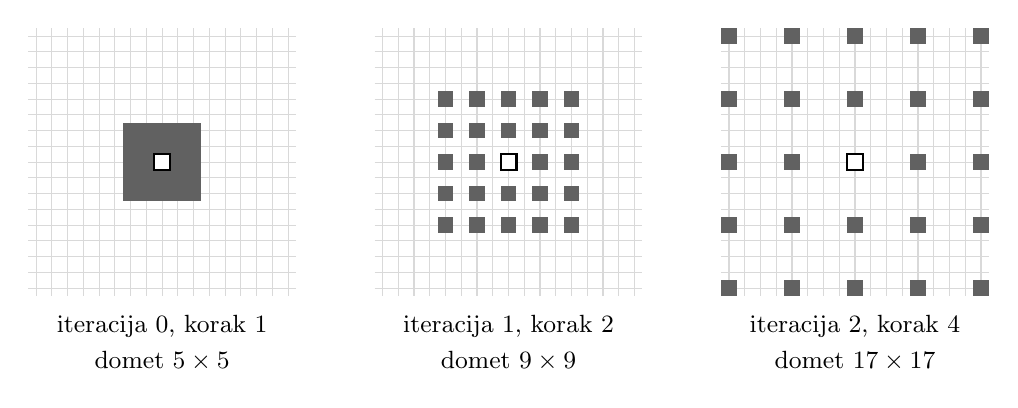
\begin{tikzpicture}[font=\scriptsize, scale=0.2]
  \foreach \it/\stride/\xoff in {0/1/0, 1/2/22, 2/4/44} {
    \begin{scope}[xshift=\xoff cm]
      \draw[black!15] (-8.5,-8.5) grid (8.5,8.5);
      \foreach \dy in {-2,-1,0,1,2} \foreach \dx in {-2,-1,0,1,2} {
        \pgfmathsetmacro{\px}{\dx*\stride}
        \pgfmathsetmacro{\py}{\dy*\stride}
        \fill[black!62] (\px-0.5,\py-0.5) rectangle (\px+0.5,\py+0.5);
      }
      \fill[white] (-0.5,-0.5) rectangle (0.5,0.5);
      \draw[black, thick] (-0.5,-0.5) rectangle (0.5,0.5);
      \node[font=\small] at (0,-10.4) {iteracija \it, korak \stride};
      \node[font=\small] at (0,-12.6) {domet $\pgfmathparse{int(4*\stride+1)}\pgfmathresult
        \times \pgfmathparse{int(4*\stride+1)}\pgfmathresult$};
    \end{scope}
  }
\end{tikzpicture}
\caption[\`A-trous: rastu\'ci korak i domet filtera]{Tri iteracije a-trous filtera, sve nad istim ise\v{c}kom $17\times17$ oko filtriranog piksela (beli kvadrat u sredini). Svaka iteracija uzima istih 25 odbiraka, samo sa duplo ve\'cim korakom, pa domet raste dok cena po iteraciji ostaje ista. Rupe izme\dj{}u odbiraka pla\'caju domet: kumulativno $29\times29$ sa 75 odbiraka umesto 841.}
\label{fig:atrous}
\end{figure}

Svaki odbirak nosi tri \v{c}lana zaustavljanja ivica (Listing~\ref{lst:atrous}): normalu, relativnu linearizovanu dubinu i \v{c}lan luminanse vo\dj{}en varijansom, koji je defini\v{s}u\'ca ideja SVGF-a. Po\v{s}to te\v{z}ina luminanse raste sa kvadratnim korenom filtrirane varijanse, filter agresivno zamu\'cuje gde je signal \v{s}umovit, a \v{c}uva detalj gde je konvergirao. Sama varijansa se filtrira kvadratima te\v{z}ina odbiraka, a svi vode\'ci baferi se uzorkuju bez interpolacije (point-sampled) da bi se izbeglo curenje preko ivica. Isklju\v{c}ivanje \v{c}lana varijanse (\texttt{LumaPhi = 0}) svodi filter na obi\v{c}an bilateralni blur, korisnu osnovnu liniju u Glavi~\ref{ch:analiza}.


\needspace{12\baselineskip}
\begin{lstlisting}[caption={Te\v{z}ine zaustavljanja ivica za \`a-trous filter (SVGF jezgro, HLSL).}, label={lst:atrous}]
float w_n = pow(saturate(dot(N, N_tap)), K_NORMAL);              // normal
float w_z = exp(-abs(z - z_tap) / (K_DEPTH * abs(dzdx) + 1e-4)); // depth
float w_l = exp(-abs(lum - lum_tap) /                            // variance-guided luminance
                (LUMA_PHI * sqrt(varBlur) + 1e-4));
float w   = w_n * w_z * w_l * kernel[dy + 2] * kernel[dx + 2];   // combined tap weight
sum  += w * color_tap;
wSum += w;
\end{lstlisting}

\subsection{Odstupanja od SVGF-a i njihova cena}

Implementacija odstupa od rada na \v{c}etiri mesta, sva navedena da bi se brojevi kvaliteta iz Glave~\ref{ch:analiza} \v{c}itali ispravno:
\begin{itemize}
\item denoiser filtrira sirovu iradijansu i ponovo mno\v{z}i albedo posle upsample-a, dok SVGF demoduli\v{s}e unutar filtera,
\item dodatni temporalni clamp boje gore nije u SVGF-u,
\item GI i AO se filtriraju u polovini rezolucije, dok je SVGF u punoj rezoluciji,
\item zaustavljanje ivica po varijansi je opciono.
\end{itemize}

Izbor na nivou izvornog koda koji ne mo\v{z}e promeniti izlaznu sliku, na primer da li je jedna petlja odmotana, odlu\v{c}uje da li \v{s}ejder dobija 16 od 16 wavefront-ova ili 8. \texttt{GIDenoise.comp} dr\v{z}i svoju spoljnu \`a-trous petlju neodmotanom, \v{s}to ko\v{s}ta malo slobode raspore\dj{}ivanja, a zauzvrat dr\v{z}i pritisak na registre na 58 VGPR-ova na RX 9070 XT, bez spilovanja i sa punom zauzeto\v{s}\'cu (Tabela~\ref{tab:occupancy}). Odmotana alocira 191, prelaze\'ci granicu alokacije koju 58 ne prelazi, i pada na 8 od 16 wavefront-ova.

\section{TAA / temporalni resolve}
\label{sec:taa}

Po\v{s}to forward prolaz proizvede osen\v{c}enu HDR sliku, temporalni anti-aliasing resolve \cite{karis2014taa} (\texttt{TemporalResolvePass}, \texttt{TemporalResolve.frag.hlsl}) akumulira je kroz frejmove da ukloni aliasing i da konvergira preostali \v{s}um koji denoiseri po efektu ostavljaju. Kamera se u svakom frejmu pomera za pod-piksel na niskodiskrepantnoj sekvenci od 16 faza, pa uzastopni frejmovi uzorkuju razli\v{c}ite ta\v{c}ke unutar piksela, a resolve reprojektuje prethodni izlaz vektorima kretanja i odseca ga prema lokalnom susedstvu trenutnog piksela, labavo za stati\v{c}an piksel i stro\v{z}e pri kretanju (d\v{z}iter je Halton(2,3), reprojekcija koristi dilataciju najbli\v{z}e dubine da tanke strukture uzmu pravu brzinu i Catmull-Rom rekonstrukciju istorije radi smanjenja zamu\'cenja reprojekcije, a odsecanje je Karis zaobljena kutija nad susedstvom $3\times3$ u YCoCg prostoru).

Resolve radi u linearnom HDR-u i samo akumulira. To je namerna invarijanta: svaka perceptivna operacija ili operacija u prostoru prikaza (izo\v{s}travanje, kontrast) dr\v{z}i se van ovog prolaza i primenjuje posle tonemap-a, jer kriva po kanalu primenjena pre tonemap-a pretvara preba\v{c}aj akumulacije u pomak nijanse. Izo\v{s}travanje zato \v{z}ivi u zasebnom prolazu posle tonemap-a, a ne ovde, i taj prolaz je podrazumevano isklju\v{c}en (\texttt{render.sharpen} 0), pa ga ni\v{s}ta izmereno u Glavi~\ref{ch:analiza} ne pokre\'ce.

Vektori kretanja su zajedni\v{c}ki preduslov tri potro\v{s}a\v{c}a: SVGF temporalnog prolaza, TAA resolve-a i screen-space efekata koji uzorkuju boju pro\v{s}log frejma. Prolaz brzine (Slika~\ref{fig:motion}) renderuje scenu drugi put i pi\v{s}e po pikselu pomak ta\v{c}ke povr\v{s}ine u prostoru ekrana izme\dj{}u prethodne i trenutne view-projection matrice.

Re\v{z}im otkaza koji ovo izla\v{z}e je disokluzija. Piksel otkriven iza okludera u ovom frejmu nema prethodnu poziciju na koju bi pokazao, pa mu je istorija bez smisla, a njeno ponovno kori\v{s}\'cenje razmazalo bi boju okludera preko novootkrivene povr\v{s}ine. Svaka temporalna faza u engine-u zato uparuje reprojekciju sa testom odbacivanja po dubini i normali, a gde se on okine, piksel se vra\'ca samo na trenutni frejm, koji je \v{s}umovitiji, ali ispravan.

\begin{figure}[tbp]
\centering

\includegraphics[width=0.8\textwidth]{figures/dbg_motion.png}
\caption[Debug prikaz vektora kretanja]{Bafer vektora kretanja (\texttt{render.debugview} 1) na \texttt{dolly} probi rute, na sceni sa animiranim rekvizitima. Crveno je horizontalni, a zeleno vertikalni pomak izme\dj{}u uzastopnih frejmova, u apsolutnoj vrednosti i skalirano sa 40, pa prikaz pokazuje intenzitet i osu, ali ne i smer. Kretanje napred daje radijalni uzorak: tamni centar je \v{z}ari\v{s}te \v{s}irenja, gde se povr\v{s}ine ka kojima se kamera kre\'ce jedva pomeraju. Pravougaone mrlje su rotiraju\'ci rekviziti, \v{c}iji se vektori prekidaju od zida iza njih, a taj prekid je gorenavedena disokluzija. Poni\v{s}tavanjem normalizacije po osi i sRGB kodiranja, srednji pomak je $0.24\%$ dijagonale ekrana, a najvi\v{s}e $0.75\%$, bez zasi\'cenog uzorka.}
\label{fig:motion}
\end{figure}

\section{Reproduktivnost i alati}
\label{sec:alati}

Merenja u Glavi~\ref{ch:analiza} poti\v{c}u iz instrumentacije ugra\dj{}ene u engine, zbog \v{c}ega su reproduktivna, a ne jednokratni snimci. Svaki efekat se uklju\v{c}uje i pode\v{s}ava kroz registar console promenljivih, pa je benchmark konfiguracija skup vrednosti CVar-ova, a ne izmena koda, podesiva iz komandne linije za headless pokretanja, a svaki prolaz grafa renderovanja obavijen je GPU timestamp opsegom. \v{C}etiri alata izgra\dj{}ena povrh toga (Tabela~\ref{tab:tooling}) porede se sa committovanom osnovnom linijom i obaraju pokretanje pri regresiji, \v{s}to i razdvaja kapiju od izve\v{s}taja: broj koji niko ne proverava lagano odlazi.

\begin{table}[tbp]
\caption[Alati za merenje]{Alati koji proizvode brojeve u Glavi~\ref{ch:analiza}. ``Kapija'' zna\v{c}i da alat poredi sa committovanom osnovnom linijom i obara pokretanje pri regresiji, dok alati bez kapije samo izve\v{s}tavaju. Svima osim \texttt{rga-occupancy} treba pravi GPU, pa rade lokalno, a ne na CI-ju.}
\label{tab:tooling}
\centering
\begin{tabular}{lp{0.55\textwidth}l}
\toprule
Alat & \v{S}ta meri & Kapija \\
\midrule
\texttt{perf-bench}     & GPU ms po prolazu, matrica konfiguracija; opciono pinovanje takta, uparena A/B presuda & da \\
\texttt{quality-bench}  & FLIP/PSNR/SSIM (LPIPS kad je dostupan) naspram path trace-a, stati\v{c}na kamera, fiksan \texttt{render.resolution} & da \\
\texttt{quality-motion} & FLIP, tFLIP, lag i JOD du\v{z} rute & da \\
\texttt{rga-occupancy}  & pritisak na registre i zauzetost, offline & da \\
\texttt{quality-tune}   & pretraga CVar-ova naspram reference & ne \\
\texttt{smoke-test}     & pad, zamrzavanje, Vulkan validacija & prolazi/pada \\
\texttt{shader-stats}   & registri koje prijavljuje drajver, oba vendora & ne \\
Tracy + watchdog        & vremenska linija po sistemu, zastoji po frejmu & ne \\
\bottomrule
\end{tabular}
\end{table}

\section{Referentni path tracer}
\label{sec:pathtracer}

Referenca je brute-force jednosmerni path tracer ugra\dj{}en u engine (\texttt{PathTrace\allowbreak.comp\allowbreak.hlsl}): next-event estimation ka suncu, isti metallic-roughness mikrofasetni BSDF kao forward \v{s}ejdiranje, vi\v{s}eodsko\v{c}no indirektno osvetljenje sa prekidom ruskom ruletom i progresivna akumulacija u trajni HDR bafer dok je kamera stati\v{c}na. Sunce se uzorkuje kao kona\v{c}an disk kroz istu \texttt{SampleCone} rutinu i isti poluugao \texttt{render.shadow.sun\_angle\_deg} kao putanja mekih senki u realnom vremenu, pa se svaka razlika u penumbri mo\v{z}e pripisati uzorkovanju i rekonstrukciji, a ne druga\v{c}ijem modelu svetla (nebo pri proma\v{s}aju zraka dodaje se bez diska sunca, da se izbegne dvostruko ra\v{c}unanje). Po\v{s}to senke, ambijentalna okluzija, refleksije i indirektno svetlo proizlaze iz istog vi\v{s}eodsko\v{c}nog transporta, jedan konvergirani path trace je ground truth za sve njih odjednom (Slika~\ref{fig:pt-ref}). Akumulira 2 putanje po pikselu po frejmu tokom najmanje 400 frejmova, dakle najmanje 800 putanja po pikselu, pri maksimalnoj du\v{z}ini putanje 8 sa prekidom ruskom ruletom, a snimak se dr\v{z}i dok ne pro\dj{}e test konvergencije, umesto da se zaustavi na fiksnom broju. Kapija ga pokre\'ce \emph{nepristrasno}, sa isklju\v{c}enim i clamp-om fireflies-a i clamp-om te\v{z}ine regularizacije putanje, jer bi clamp-ovana referenca pristrasila upravo energiju prema kojoj se tehnike u realnom vremenu ocenjuju. Postoji samo kao oslonac ispravnosti. Obe strane svakog pore\dj{}enja prolaze kroz isti tonemap lanac, pa je uklju\v{c}ivanje path tracer-a A/B pore\dj{}enje jabuka sa jabukama, a ne pore\dj{}enje HDR i LDR slike.

\begin{figure}[tbp]
\centering
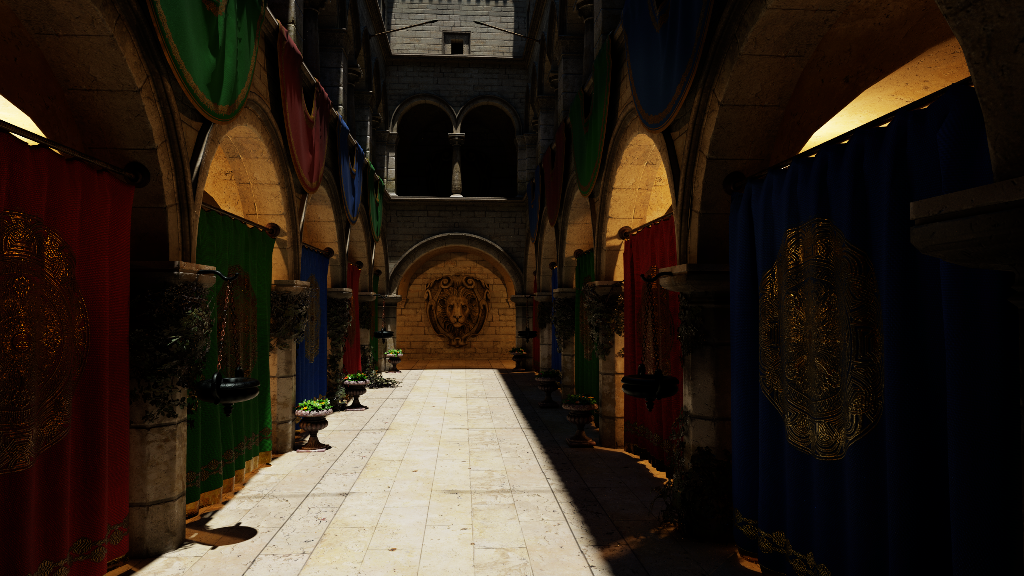
\includegraphics[width=0.85\textwidth]{figures/pt_ref.png}
\caption[Konvergirani referentni frejm path tracer-a]{Konvergirani referentni frejm ugra\dj{}enog path tracer-a, prema kome se svaka tehnika u realnom vremenu meri preko FLIP/PSNR/SSIM.}
\label{fig:pt-ref}
\end{figure}

\section{Uslovi i pretpostavke}
\label{sec:uslovi}

Implementacija pravi nekoliko namernih aproksimacija da ostane u bud\v{z}etu realnog vremena, svaka je pojednostavljenje punog problema, a ne faktor koji iskrivljuje relativna merenja u Glavi~\ref{ch:analiza}.

\begin{itemize}
  \item \textbf{Difuzno GI sa jednim odskokom.} Globalno osvetljenje ra\v{c}una jedan difuzni indirektni odskok, dok su vi\v{s}eodsko\v{c}no i sjajno indirektno osvetljenje van opsega.
  \item \textbf{GI i AO u polovini rezolucije.} GI i AO se prate u polovini rezolucije i bilateralno upsample-uju. Refleksije se prate u punoj rezoluciji.
  \item \textbf{Mali broj uzoraka uz rekonstrukciju.} Efekti koriste jedan ili dva zraka po pikselu i za upotrebljivu sliku zavise od temporalne akumulacije, a za GI i AO i od prostornog SVGF filtera. Prostorni filter je za refleksije isklju\v{c}en (Odeljak~\ref{sec:denoise-eval}).
  \item \textbf{Pribli\v{z}ne meke senke.} U podrazumevanoj putanji senke pra\'cenjem zraka koriste jedan tvrd ili dva meka zraka po svetlu, prate se inline i primenjuju direktno bez denoisera, pa je penumbra dvouzorkovna aproksimacija povr\v{s}inskog svetla koju \v{c}isti samo temporalni resolve, a ne konvergirana meka senka. Opciona stohasti\v{c}ka putanja rekonstrui\v{s}e svoju agregatnu vidljivost kroz zajedni\v{c}ki denoiser, po ceni razre\v{s}avanja samo jednog svetla po pikselu po frejmu.
  \item \textbf{Samo inline ray query-ji.} Nema ray tracing pipeline-a, shader binding table-a ni rekurzije. Svo osvetljenje pogotka je jedan odskok evaluiran u \texttt{ShadeSurfaceHit}.
  \item \textbf{NEE lokalnih svetala sa jednim uzorkom, samo GI.} Sekundarni pogodak GI dodaje najvi\v{s}e jedno od ta\v{c}kastih i spot svetala scene, izabrano importance sampling-om po pogotku, a ne sumirano preko svih, pa ostaje \v{s}umovit estimator sa jednim uzorkom pune next-event estimation, a ne ta\v{c}na suma. Pogoci refleksija uop\v{s}te nisu pro\v{s}ireni lokalnim svetlima (\texttt{render.rt.hit_lights} nije izmerio dobitak kvaliteta tu za dvostruku cenu na GI strani).
  \item \textbf{Potpuna ponovna izgradnja TLAS-a po dinami\v{c}nom frejmu.} Struktura najvi\v{s}eg nivoa ponovo se gradi, a ne osve\v{z}ava, u svakom frejmu u kom se scena menja, iako potpuno stati\v{c}na scena preska\v{c}e ponovnu izgradnju.
\end{itemize}
